% -*- mode: latex; mode: reftex; mode: auto-fill; mode: flyspell; coding: utf-8; tex-command: "pdflatex.sh" -*-

\documentclass[oneside,11pt]{memoir}

\input{layout.tex}


\usepackage{lipsum} 

\hypersetup{
  pdfauthor={Abel Hernández},
  pdftitle={Documento_prac},
  pdfsubject={xxxxxx},
  pdfkeywords={xxxxxx},
  pdfproducer={LaTeX and TikZ},
  pdfcreator={pdflatex},
}

%%%%%%%%%%%%%%%%%%%%%%%%%%%%%%%%%%%%%%%%%%%%%%%%%%%%%%%%%%%%%%%%%%%%%%%%%%%%%%%%%%%%%%%%%%%

\begin{document}

\thispagestyle{empty}

\begin{center}

\vspace*{\stretch{1}}

{\huge Geometría diferencial\\[0.75ex] de curvas y superficies}

\vspace*{4ex}

Notas del verano académico IMPA 2024\\

\vspace*{5 ex}


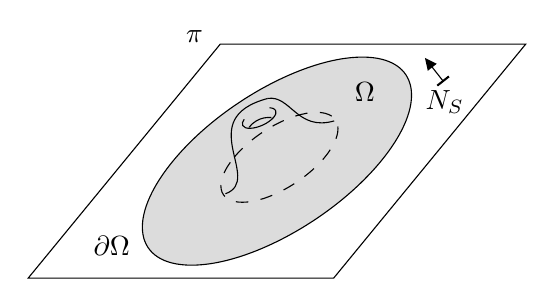
\begin{tikzpicture}[x=0.6pt,y=0.6pt,yscale=-1,xscale=1]
%uncomment if require: \path (0,300); %set diagram left start at 0, and has height of 300

%Shape: Ellipse [id:dp7174187445582809] 
\draw  [fill={rgb, 255:red, 155; green, 155; blue, 155 }  ,fill opacity=0.35 ] (254.19,142.55) .. controls (282.6,107.95) and (333.67,79.89) .. (368.28,79.89) .. controls (402.88,79.89) and (407.91,107.95) .. (379.51,142.55) .. controls (351.1,177.15) and (300.02,205.21) .. (265.42,205.21) .. controls (230.82,205.21) and (225.79,177.15) .. (254.19,142.55) -- cycle ;
%Shape: Rectangle [id:dp5888300228311276] 
\draw   (282.68,72.12) -- (466.64,72.12) -- (351.02,212.98) -- (167.06,212.98) -- cycle ;
%Shape: Ellipse [id:dp8780839153902946] 
\draw  [dash pattern={on 4.5pt off 4.5pt}] (291.08,140.25) .. controls (303.44,125.29) and (325.66,113.17) .. (340.71,113.17) .. controls (355.76,113.17) and (357.95,125.29) .. (345.59,140.25) .. controls (333.24,155.2) and (311.02,167.32) .. (295.97,167.32) .. controls (280.92,167.32) and (278.73,155.2) .. (291.08,140.25) -- cycle ;
%Curve Lines [id:da4915332848369254] 
\draw    (285.83,162.21) .. controls (309.11,153.75) and (265.65,117.06) .. (311.25,104.81) ;
%Curve Lines [id:da8579079241038665] 
\draw    (311.25,104.81) .. controls (325.08,102.56) and (328.95,124.79) .. (351.34,118.32) ;
%Shape: Arc [id:dp27687929601806816] 
\draw  [draw opacity=0] (312.37,110.36) .. controls (314.18,110.43) and (315.53,110.98) .. (316.07,112.01) .. controls (317.29,114.34) and (313.84,118.28) .. (308.37,120.8) .. controls (302.9,123.32) and (297.47,123.46) .. (296.26,121.13) .. controls (295.72,120.1) and (296.09,118.76) .. (297.13,117.37) -- (306.16,116.57) -- cycle ; \draw   (312.37,110.36) .. controls (314.18,110.43) and (315.53,110.98) .. (316.07,112.01) .. controls (317.29,114.34) and (313.84,118.28) .. (308.37,120.8) .. controls (302.9,123.32) and (297.47,123.46) .. (296.26,121.13) .. controls (295.72,120.1) and (296.09,118.76) .. (297.13,117.37) ;  
%Shape: Arc [id:dp17382975760483887] 
\draw  [draw opacity=0] (300.06,122.19) .. controls (301.21,120.63) and (302.72,119.27) .. (304.56,118.22) .. controls (307.33,116.64) and (310.43,116.03) .. (313.43,116.26) -- (312.19,130.06) -- cycle ; \draw   (300.06,122.19) .. controls (301.21,120.63) and (302.72,119.27) .. (304.56,118.22) .. controls (307.33,116.64) and (310.43,116.03) .. (313.43,116.26) ;  
%Straight Lines [id:da37298789113540876] 
\draw    (416.91,94.31) -- (407.83,82.78) ;
\draw [shift={(405.98,80.42)}, rotate = 51.8] [fill={rgb, 255:red, 0; green, 0; blue, 0 }  ][line width=0.08]  [draw opacity=0] (7.14,-3.43) -- (0,0) -- (7.14,3.43) -- cycle    ;
\draw [shift={(416.91,94.31)}, rotate = 51.8] [color={rgb, 255:red, 0; green, 0; blue, 0 }  ][line width=0.75]    (0,4.47) -- (0,-4.47)   ;

% Text Node
\draw (362.24,93.91) node [anchor=north west][inner sep=0.75pt]    {$\Omega $};
% Text Node
\draw (404.83,98.49) node [anchor=north west][inner sep=0.75pt]    {$N_{S}$};
% Text Node
\draw (260.57,62.51) node [anchor=north west][inner sep=0.75pt]    {$\pi $};
% Text Node
\draw (204.93,186.33) node [anchor=north west][inner sep=0.75pt]    {$\partial \Omega $};


\end{tikzpicture}
\vspace*{0.3 cm}\\
\footnotesize{Abel Hernández} 
\vspace*{\stretch{0.8}}\\
\begin{center}
    \includegraphics[scale=0.22]{figuras/escudo2.jpg}
    \hspace{1.4 cm}
    \includegraphics[scale=0.13]{figuras/escudo1.png}
\end{center}

\end{center}

\newpage

%%%%%%%%%%%%%%%%%%%%%%%%%%%%%%%%%%%%%%%%%%%%%%%%%%%%%%%%%%%%%%%%%%%%%%%%%%%%%%%%%%%%%%%%%%%

\vspace*{\stretch{1.}}

Estas notas fueron optimizadas para mostrarse en dispositivos móviles.

\vspace*{\stretch{1}}



\vspace*{-3ex}

\newpage

%%%%%%%%%%%%%%%%%%%%%%%%%%%%%%%%%%%%%%%%%%%%%%%%%%%%%%%%%%%%%%%%%%%%%%%%%%%%%%%%%%%%%%%%%%%
% Table of content
%%%%%%%%%%%%%%%%%%%%%%%%%%%%%%%%%%%%%%%%%%%%%%%%%%%%%%%%%%%%%%%%%%%%%%%%%%%%%%%%%%%%%%%%%%%

{
\everymath{\color{black}}
\tableofcontents* % Prints the table of contents
%\addcontentsline{toc}{chapter}{Contents}
}

\clearpage



%%%%%%%%%%%%%%%%%%%%%%%%%%%%%%%%%%%%%%%%%%%%%%%%%%%%%%%%%%%%%%%%%%%%%%%%%%%%%%%%%%%%%%%%%%%

\chapter*{Prefacio}
\addcontentsline{toc}{chapter}{Prefacio}
En el año 2024, fue impartido el curso ``\textit{Geometria Diferencial de Curvas e Superfícies}'' dentro del IMPA de la mano del investigador Lucas Ambrozio; siendo este curso parte del programa de verano académico. Dicho programa brinda un primer acercamiento a matemáticas de posgrado a estudiantes de licenciatura que deseen aventurarse en el mundo de la investigación en matemáticas puras. En concreto el curso presentó la teoría básica sobre curvas y superficies, así como algunos temas de investigación del doctor Lucas. Dentro de la Escuela de ciencias físicas y matemáticas de la USAC, a la fecha existen escasos registros de estudiantes en este programa, por lo que es importante la creación de este tipo de textos que dejen constancia de la participación de la escuela en estas instituciones.

El siguiente material contiene temas poco convencionales tratados dentro del curso, traduciendo del portugués los materiales complementarios del profesor, así como algunas soluciones de problemas propuestos dentro del curso. Adicionalmente también se agregaron ejercicios de la lista grande, siendo esta un problemario brindado al inicio del verano como referencia para las pruebas del curso.

El estudio de la geometría diferencial va de la mano con al análisis de variable real, la topología y el álgebra lineal, pues muchos conceptos como superficies y variedades se definen en función de espacios topológicos y la definición de algunos mapeos dentro de superficies pueden ser analizados como transformaciones lineales. Por ello estas notas, a parte de ser una descripción de una ruta sólida para un primer curso de geometría diferencial, se presentan resultados que usualmente no se tratan en los libros convencionales, algunos de estos resultados son del análisis de Fourier y del álgebra lineal avanzada.


La parte de geometría plana (en $\mathbb{R}^2$) contiene resultados, ejemplos y pruebas necesarias dentro de un curso de geometría diferencial siendo los primeros dos capítulos importantes y detallados. En el capítulo 3 y 4, se presentan algunas definiciones importantes y referencias fundamentales para un curso, sin embargo se omite el desarrollo riguroso de la teoría para presentar detalles y contraejemplos muy concretos que aportan a la lectura de la bibliografía recomendada. En el capítulo 5 se presenta un resultado no tan conocido y que para algunos podrá parecer bastante simple, que sin embargo se recomienda leer para entender a profundidad el conocido como el teorema fundamental de curvas en el espacio, siendo este un capítulo complementario a las lecturas recomendadas. Finalmente el capítulo 6 presenta un problema propuesto dentro del curso del IMPA y posee ideas fundamentales de aplicaciones de Gauss Bonnet así como una generalización del teorema cuyo nombre es el mismo que el del capítulo. Con este último capítulo si se recomienda una revisión rigurosa de las lecturas sugeridas pues el contenido es un poco avanzado y requiere herramientas de análisis más sofisticadas.

\chapter*{Generalidades y prerrequisitos}
\addcontentsline{toc}{chapter}{Generalidades y prerrequisitos}

En el siguiente capítulo se presentarán algunas convenciones usadas en el resto del texto y se proponen algunos ejercicios a manera de prerrequisito para abordar un curso de geometría diferencial a nivel de pregrado o licenciatura. Algunos de los ejercicios usan teoría de álgebra lineal, cálculo de varias variables y teoría de grupos.
\\
Se agregaron algunos ejercicios prescindibles para abordar el curso, pero que no dejan de ser resultados curiosos para un lector que ya haya tenido contacto previo con la materia.



\section{Notación}
\begin{definition}
Si $p=(x^1,x^2,...,x^n)$ y $q=(y^1,y^2,...,y^n)$, elementos de $\mathbb{R}^n$, se define
\begin{align*}
    \langle p,q \rangle =\sum_{i=1}^nx^iy^i
\end{align*}
como el \textbf{producto interno euclideano} en $\mathbb{R}^n$.
\end{definition}

\begin{definition}\label{metrica}
Si $p,q\in \mathbb{R}^n$, se define
\begin{align*}
    d(p,q)  =\sqrt{\langle p-q,p-q \rangle}=|p-q|
\end{align*}
la \textbf{distancia euclideana} en $\mathbb{R}^n$.
\end{definition}
Siendo esta la manera usual en la que medimos distancias en $\mathbb{R}^n$. Con esto podemos medir ángulos entre vectores de la siguiente forma: Si $p,q\in \mathbb{R}^n$, son dos elementos no nulos de $\mathbb{R}^n$, se tiene
\begin{align*}
    \cos \theta =\left\langle \dfrac{p}{|p|},\dfrac{q}{|q|}\right\rangle
\end{align*}
 Las siguientes identidades muestran que, de hecho, las medidas de ángulos se puede reducir a medidas de distancia.
\begin{proposition}
    Para cualesquiera $x$ e $y$ en $\mathbb{R}^n$, valen las siguientes identidades
    \begin{align*}
        \langle x,y \rangle&= \dfrac{1}{4}|x+y|^2-\dfrac{1}{4}|x-y|^2\\
        \langle x,y \rangle&= \dfrac{1}{2}\left(|x+y|^2-|x|^2-|y|^2\right)
    \end{align*}
\end{proposition}
Desde un punto de vista geométrico, es fundamental clasificar las simetrías del espacio euclidiano,
es decir, las transformaciones que preservan su geometría, por lo que es importante fijarnos en las siguientes funciones
\begin{definition}
    Decimos que una transformación $\phi:\mathbb{R}^n\to \mathbb{R}^n$ \textbf{preserva distancias} si    
    \begin{align*}
        |\phi(x)-\phi(y)|=|x-y| \quad \forall\text{ } x,y\in \mathbb{R}^n
    \end{align*}
\end{definition}
Podemos verificar que las traslaciones $T_v(p)=p+v$ con $p\in \mathbb{R}^n$ fijo, preservan distancias, de igual manera las transformaciones lineales del grupo $O(n)$, es decir, las transformaciones ortogonales.

El espacio euclidiano tiene una estructura extra, la cual es su orientación canónica definida por su base canónica $\{e_1,\ldots, e_n\}$. Distinguiremos entonces el subconjunto $SO(n)$ de $O(n)$ formado por todas las transformaciones ortogonales que \textbf{preservan la orientación} de $\mathbb{R}^n$. Más concretamente diremos que $R\in SO(n)$ si y solamente si $R\in O(n)$ y la matriz de cambio de base de $\{e_1,\ldots, e_n\}$ a $\{Re_1,\ldots, Re_n\}$ tiene determinante positivo. Para más sobre la orientación de $\mathbb{R}^n$ puede consultarse el apéndice A.\\

Concluyendo con la estructura geométrica de el espacio $\mathbb{R}^n$, definiremos unos objetos importantes dentro de las transformaciones del espacio euclidiano 
\begin{definition}
    Decimos que $M:\mathbb{R}^n\to \mathbb{R}^n$ es un movimiento rígido si es la composición de un número finito de translaciones y elementos de $SO(n)$.
\end{definition}

 En un contexto más topológico, si regresamos a la definición \ref{metrica}, tendremos que $d$ es una métrica, funciones las cuales son estudiadas en un primer curso de  análisis de variable real y define junto a $\mathbb{R}^n$ un espacio métrico del cual estas son algunas de sus propiedades
\begin{proposition}
Con la notación anteriormente usada:
    \begin{enumerate}
        \item $(\mathbb{R}^n,d)$ es un espacio métrico completo. Es decir toda sucesión de Cauchy es convergente.
        \item Si $ \mathbb{R}^n$ es visto como espacio topológico junto con los abiertos generados por la métrica $d$. Este espacio topológico tiene una base contable.
    \end{enumerate}
\end{proposition}
Estas propiedades lo que nos indican es que $\mathbb{R}^n$ con su estructura topológica no tiene ``demasiados abiertos'' y por otro lado, que no tendremos ``agujeros'' como los que tienen los racionales en los reales.
\section{Ejercicios}
\subsection{Prerrequisitos}
\textcolor{blue}{\textbf{0.1.}} Enuncie los axiomas de un espacio vectorial (real). Indique la definición de una norma. Defina  producto interno y norma inducida. Demuestre que si la norma $|\cdot|$ está inducida por un producto interno $\langle\cdot,\cdot\rangle$, entonces verifica la identidad del paralelogramo
    \begin{align*}
        |x+y|^2+|x-y|^2=2|x|^2+2|y|^2
    \end{align*}
¿El converso es cierto?

\textcolor{blue}{\textbf{0.2.}} Considere un espacio vectorial real $V$, dotado de un producto interno $\langle\cdot,\cdot\rangle$. Defina base ortonormal, $\{v_1,\ldots,v_n\}$ de $V$. Si expresamos un vector arbitrario $v\in V$ en esta base como
\begin{align*}
    v=\sum_{i=1}^na^iv_i
\end{align*}
use el producto interno para calcular los coeficientes $a^i$ y $|v|^2$ en función de estos $a^i$.

\textcolor{blue}{\textbf{0.3.}} Bajo las mismas hipótesis que en el ejercicio anterior, sea $v\neq 0$ en $V$. Usando el producto interno, escriba la fórmula para la proyección ortogonal de un punto $p\in V$ en el subespacio generado por $v$, y la fórmula para la proyección ortogonal de un punto $p\in V$ en el complemento ortogonal del subespacio generado por $v$.

\textcolor{blue}{\textbf{0.4.}} Considere la aplicación lineal 
\begin{align*}
    J:\mathbb{R}^2&\to \mathbb{R}^2\\
    (a,b)&\mapsto (-b,a).
\end{align*}
Describa esta aplicación geométricamente y muestre que
\begin{enumerate}
    \item[$i)$] $J^2=-I_2$
    \item[$ii)$] $\langle Jx, Jy \rangle = \langle x,y\rangle$ para todos $x,y\in \mathbb{R}^2$.
\end{enumerate}
¿Existe un endomorfismo lineal de $\mathbb{R}^3$ que satisface $i)$ y $ii)$? ¿En $\mathbb{R}^4$?

\textcolor{blue}{\textbf{0.5.}} Sean $\alpha,\beta:I\to \mathbb{R}^n$ funciones suaves (= de la clase $C^\infty$).
\begin{enumerate}
    \item[$i)$] Mostrar que la aplicación $t\in I\to \langle\alpha(t),\beta(t)\rangle \in \mathbb{R}$ es suave y calcule su derivada.
    \item[$ii)$] Mostrar que la aplicación $t\in I\to |\alpha(t)| \in \mathbb{R}$ es continua en $I$ y suave excepto los puntos $t\in I$ donde $\alpha(t)=0$. Calcule la derivada en los puntos en los que existe.
    \item[$iii)$] Suponga que la imagen de $\alpha$ no contiene el origen, y que $\alpha(t_0)$, $t_0\in I$ es el punto de $\alpha(I)$ más cercano al origen. Mostrar que $\alpha'(t_0)$ es ortogonal a $\alpha(t_0)$.
\end{enumerate}

\textcolor{blue}{\textbf{0.6.}}  Sea $L:\mathbb{R}^m\to \mathbb{R}$ una aplicación lineal. Muestre que existe un único vector $v_0\in\mathbb{R}^m$ tal que
\begin{align*}
    L(w)=\langle v_0,w\rangle \quad \forall w\in\mathbb{R}^m.
\end{align*}

\textcolor{blue}{\textbf{0.7.}} Sea $V$ un espacio vectorial real de dimensión finita, dotado de un producto interno. La transformación adjunta de una transformación lineal $A:V\to V$ es la transformación $A^*:V\to V$ que asocia cada $x\in V$ a un único punto $A^*x\in V$ tal que
\begin{align*}
    \langle A^*x,y\rangle= \langle x,Ay\rangle \quad \text{ para todo }y\in V.
\end{align*}
Explique porque $A^*$ está bien definida y muestre que la transformación $J$ definida en el ejercicio 0.4 satisface $J^*=J^{-1}=-J$.

\textcolor{blue}{\textbf{0.8.}} Una transformación autoadjunta (o simétrica) de un espacio vectorial real $V$
de dimensión finita dotado de un producto interno es una aplicación lineal $A:V\to V$ tal que $A=A^*$.
\begin{enumerate}
    \item[$i)$] El teorema espectral para operadores autoadjuntos establece que para todas las transformaciones
 autoadjuntas $A$ hay una base ortonormal $\{v_1,\ldots,v_n\}$ que las diagonaliza, esto es, existen $\lambda_i\in \mathbb{R}$ tales que $Av_i=\lambda_iv_i$ para todo $i=1,\ldots,n$. Relacione este enunciado con la versión que conoce del teorema espectral.
    \item[$ii)$] Considerando $A:\mathbb{R}^n\to \mathbb{R}^n$ lineal y autoadjunta, muestre que la función 
    \begin{align*}
        Q:\mathbb{R}^n\times \mathbb{R}^n&\to \mathbb{R}\\
        (x,y)&\mapsto \langle Ax, y\rangle 
    \end{align*}
    es bilineal y simétrica. Calcular los puntos críticos y valores críticos de la función
    \begin{align*}
        f&:\mathbb{R}^n-\{0\}\to \mathbb{R}\\
        f&(x)= \dfrac{Q(x,x)}{\langle x,x\rangle}
    \end{align*}
\end{enumerate}

\textcolor{blue}{\textbf{0.9.}} Sea $X$ un subconjunto de $\mathbb{R}^n$. Defina lo que significa que $X$ es un subconjunto
abierto/cerrado/compacto/conexo/conexo por caminos/acotado. Dar ejemplos de
subconjuntos $X$ que satisfacen estas propiedades y que no las satisfacen.

\textcolor{blue}{\textbf{0.10.}} Sea $f:K\subseteq \mathbb{R}^m\to \mathbb{R}^n$ una aplicación continua e inyectiva definida en un compacto. Muestre que la inversa $f^{-1}:f(K)\to K$ está bien definida y es también continua.

\textcolor{blue}{\textbf{0.11.}} Sea $F:U\subseteq \mathbb{R}^m\to \mathbb{R}^n$ una función suave definida en un abierto $U$. Explique como se define la derivada de $F$ en un punto $p\in U$, vista como una transformación lineal $DF(p):\mathbb{R}^m\to \mathbb{R}^n$. Escriba la regla de la cadena para la composición $G\circ F$ de funciones suaves $F:U\subseteq \mathbb{R}^m\to \mathbb{R}^n$ y $G:V\subseteq \mathbb{R}^n\to \mathbb{R}^p$ con $F(U)\subseteq V$.

\textcolor{blue}{\textbf{0.12.}} \textit{(Un ejercicio en álgebra lineal y diferenciación)}
\begin{enumerate}
    \item[$i)$] Una aplicación lineal $L:\mathbb{R}\to\mathbb{R}^n$ es idénticamente nula o inyectiva.
    \item[$ii)$] Sea $F:I\subseteq \mathbb{R}\to\mathbb{R}^n$ una aplicación suave definida en un intervalo abierto $I$, $t$ un punto de $I$, y $DF(t):\mathbb{R}\to\mathbb{R}^n$ la derivada de $F$ en un punto $t$ (vista como aplicación lineal). Si $F(t)=(F^1(t),\ldots,F^n(t))$, $t\in \mathbb{R}$ es una expresión de $F$ en coordenadas, muestre que
    \begin{align*}
        DF(t)\cdot 1 =((F^1)'(t),\ldots,(F^n)'(t)).
    \end{align*}
    Nota: Tener cuidado con los detalles y la notación, $1$ es el vector que genera a $\mathbb{R}$ como espacio vectorial real.
    \item[$iii)$] Una aplicación lineal $L:\mathbb{R}^m\to\mathbb{R}$ es idénticamente nula o sobreyectiva.
    \item[$iv)$] Sea $F:U\subseteq \mathbb{R}^m\to \mathbb{R}$ una aplicación suave definida en un abierto $U$, $p=(x^1,\ldots,x^m)$ un punto de $U$, y $DF(p):\mathbb{R}^m\to \mathbb{R}$ la derivada de $F$ en un punto $p$. Muestre que el único vector asociado a esta aplicación lineal definido como en el ejercicio 0.6, es precisamente el vector
    \begin{align*}
        \text{grad }F(p):=\left(\dfrac{\partial F}{\partial x^1}(p),\ldots,\dfrac{\partial F}{\partial x^m}(p)\right) 
    \end{align*}
    más conocido como el vector gradiente de $F$ en un punto $p\in U$.
\end{enumerate}
\textcolor{blue}{\textbf{0.13.}} \textit{(Funciones $C^\infty$ de soporte compacto)}
\begin{enumerate}
    \item[$i)$] Considere la función $\eta:\mathbb{R}\to \mathbb{R}$ que se anula en puntos $t\leq 0$ y que está dada por $\eta(t)=e^{-1/t}$ si $t>0$. Muestre que esta función es de la clase $C^\infty$ ¿Es analítica?
    \item[$ii)$] Sea $\phi:\mathbb{R}^n\to \mathbb{R}$ una función que se anula fuera de la bola abierta unitaria centrada en el origen y está dada por $\phi(p)=e^{-1/(1-|p|^2)}$ si $|p|<1$. Muestre que $\phi$ es una función de la clase $C^\infty$, no negativa, y que su \textit{soporte}\footnote{El soporte se define como la cerradura del conjunto en donde es diferente de cero} es un conjunto compacto no vacío.
\end{enumerate}
\subsection{Movimientos rígidos}

%%%%%%%%%%%%%%%%%%%%%%%%%%%%%%%%%%%%%%%%%%%%%%%%%%%%%%%%%%%%%%%%%%%%%%%%%%%%%%%%%%%%%%%%%%%

\part{Geometría en $\mathbb{R}^2$ }


%% This first part provides a minimal background about machine
%% learning, issues and techniques for efficient computation, and the
%% strategies to train a parametric model.

%%%%%%%%%%%%%%%%%%%%%%%%%%%%%%%%%%%%%%%%%%%
\chapter{Curvas planas}
El estudio de las curvas planas como objetos unidimensionales es sumamente importante para el desarrollo de la geometría diferencial, pues la teoría desarrollada en este contexto particular nos ayuda obtener la intuición para generalizar  resultados a $\mathbb{R}^3$ y $\mathbb{R}^n$.\\

Si se desea profundizar en estos temas se recomienda el primer capítulo de \cite{do2016differential} y el primer capítulo de \cite{montiel2009curves}, siendo este último libro portador de varios ejercicios con mayor dificultad que la de un texto introductorio.

\section{Curvas parametrizadas regulares}
La definición que se tomará para un curva regular parametrizada, no será como un cierto subconjunto de $\mathbb{R}^n$, si no como una aplicación de la recta real al espacio euclidiano de dimensión $n$. En este contexto, consideraremos a $I$ como un intervalo abierto a partir de ahora.
\begin{figure}[h]
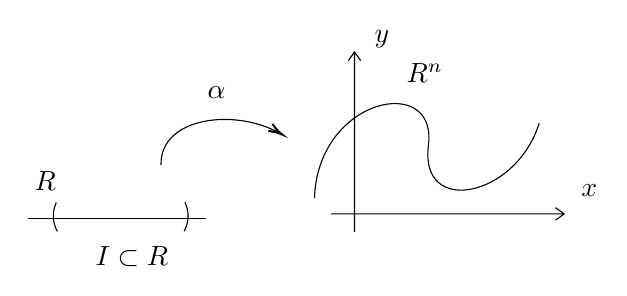
\begin{tikzpicture}[x=0.45pt,y=0.45pt,yscale=-1,xscale=1]
%uncomment if require: \path (0,300); %set diagram left start at 0, and has height of 300

%Straight Lines [id:da9928970195386473] 
\draw    (106,200.96) -- (248.68,200.96) ;
%Shape: Axis 2D [id:dp4255682573610562] 
\draw  (349.28,197.6) -- (536.41,197.6)(367.99,67.58) -- (367.99,212.05) (529.41,192.6) -- (536.41,197.6) -- (529.41,202.6) (362.99,74.58) -- (367.99,67.58) -- (372.99,74.58)  ;
%Curve Lines [id:da7310866572673476] 
\draw    (335.85,185.02) .. controls (338.44,103.83) and (434.91,84.54) .. (427.36,142.42) .. controls (419.81,200.31) and (497.82,184.37) .. (516.28,124.81) ;
%Shape: Arc [id:dp9489508685021768] 
\draw  [draw opacity=0] (129.38,211.65) .. controls (125.47,204.72) and (124.96,196.09) .. (128.55,188.53) -- (151.3,199.28) -- cycle ; \draw   (129.38,211.65) .. controls (125.47,204.72) and (124.96,196.09) .. (128.55,188.53) ;  
%Shape: Arc [id:dp10253294893661224] 
\draw  [draw opacity=0] (231.83,188.31) .. controls (235.3,195.48) and (235.27,204.11) .. (231.22,211.44) -- (209.18,199.28) -- cycle ; \draw   (231.83,188.31) .. controls (235.3,195.48) and (235.27,204.11) .. (231.22,211.44) ;  
%Curve Lines [id:da4399621105086198] 
\draw    (212.6,158.36) .. controls (211.84,119.71) and (272,112.44) .. (308.21,132.9) ;
\draw [shift={(309.85,133.85)}, rotate = 210.99] [color={rgb, 255:red, 0; green, 0; blue, 0 }  ][line width=0.75]    (10.93,-3.29) .. controls (6.95,-1.4) and (3.31,-0.3) .. (0,0) .. controls (3.31,0.3) and (6.95,1.4) .. (10.93,3.29)   ;

% Text Node
\draw (548.01,171.66) node [anchor=north west][inner sep=0.75pt]    {$x$};
% Text Node
\draw (382.14,48.52) node [anchor=north west][inner sep=0.75pt]    {$y$};
% Text Node
\draw (108.99,161.48) node [anchor=north west][inner sep=0.75pt]    {$\mathbb{R}$};
% Text Node
\draw (407.82,75) node [anchor=north west][inner sep=0.75pt]    {$\mathbb{R}^{n}$};
% Text Node
\draw (157.99,221.48) node [anchor=north west][inner sep=0.75pt]    {$I\subset \mathbb{R}$};
% Text Node
\draw (248,93.4) node [anchor=north west][inner sep=0.75pt]    {$\alpha $};
\end{tikzpicture}
\caption{Curva parametrizada para $n=2.$}
\end{figure}

La siguiente definición se da para $\mathbb{R}^n$ debido a que es una generalización natural.
\begin{definition}
    Una \textbf{curva parametrizada regular} en $\mathbb{R}^n$ es una aplicación suave\footnote{Es decir, de clase $C^\infty$} $\alpha:I\subset \mathbb{R}\to \mathbb{R}^n$ tal que $\alpha'(t)\neq 0$ para todo $t\in I$.
    \begin{itemize}
        \item A los $t\in I$ los llamaremos parámetros.
        \item $\alpha'(t)$ es el vector tangente/velocidad de $\alpha$ en $t\in I$.
        \item A $\alpha(I)\subset \mathbb{R}^n$, le llamaremos trazo, gráfico o imagen de $\alpha$. 
    \end{itemize}
\end{definition}
Otra propiedad que podemos definir con la generalidad de $\mathbb{R}^n$ desde ya, es la de una reparametrización y la de longitud de arco. Dados dos intervalos abiertos $I$ y $J$ en $\mathbb{R}$, un difeomorfismo suave $\phi: J \to I$, y una curva $\alpha : I \to \mathbb{R}^3$, podemos considerar una nueva curva $\beta: J \to \mathbb{R}^3$ definida por
la composición $\beta = \alpha \circ\phi$, vistas en \ref{fig:reparametrización}.
\begin{figure}[h]
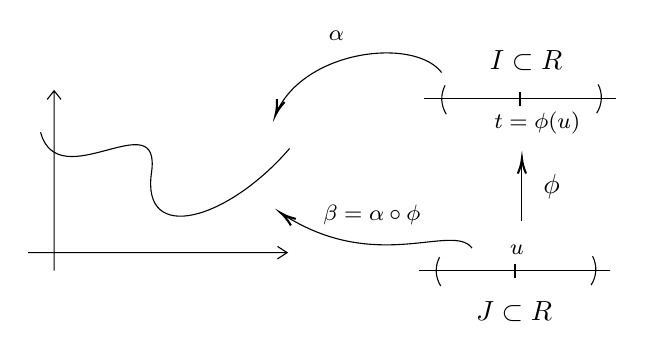
\begin{tikzpicture}[x=0.5pt,y=0.45pt,yscale=-1,xscale=1]
%uncomment if require: \path (0,300); %set diagram left start at 0, and has height of 300

%Shape: Axis 2D [id:dp39124293731149873] 
\draw  (89.28,200.6) -- (276.41,200.6)(107.99,70.58) -- (107.99,215.05) (269.41,195.6) -- (276.41,200.6) -- (269.41,205.6) (102.99,77.58) -- (107.99,70.58) -- (112.99,77.58)  ;
%Curve Lines [id:da5191307590141301] 
\draw    (98.2,103.94) .. controls (111.2,156.94) and (185.91,78.54) .. (178.36,136.42) .. controls (170.81,194.31) and (233.2,174.94) .. (278.2,116.94) ;
%Straight Lines [id:da9720087830507471] 
\draw    (375.64,77) -- (514,77) ;
\draw [shift={(444.82,77)}, rotate = 180] [color={rgb, 255:red, 0; green, 0; blue, 0 }  ][line width=0.75]    (0,5.59) -- (0,-5.59)   ;
%Shape: Arc [id:dp7031239327736214] 
\draw  [draw opacity=0] (391.38,89.39) .. controls (387.47,82.45) and (386.96,73.83) .. (390.55,66.26) -- (413.3,77.02) -- cycle ; \draw   (391.38,89.39) .. controls (387.47,82.45) and (386.96,73.83) .. (390.55,66.26) ;  
%Shape: Arc [id:dp4162311653476929] 
\draw  [draw opacity=0] (501.17,65.51) .. controls (504.49,72.75) and (504.29,81.38) .. (500.08,88.63) -- (478.3,76.02) -- cycle ; \draw   (501.17,65.51) .. controls (504.49,72.75) and (504.29,81.38) .. (500.08,88.63) ;  
%Straight Lines [id:da4342372173525715] 
\draw    (371.64,215) -- (510,215) ;
\draw [shift={(440.82,215)}, rotate = 180] [color={rgb, 255:red, 0; green, 0; blue, 0 }  ][line width=0.75]    (0,5.59) -- (0,-5.59)   ;
%Shape: Arc [id:dp04712842452226762] 
\draw  [draw opacity=0] (387.38,227.39) .. controls (383.47,220.45) and (382.96,211.83) .. (386.55,204.26) -- (409.3,215.02) -- cycle ; \draw   (387.38,227.39) .. controls (383.47,220.45) and (382.96,211.83) .. (386.55,204.26) ;  
%Shape: Arc [id:dp3268623578328633] 
\draw  [draw opacity=0] (497.17,203.51) .. controls (500.49,210.75) and (500.29,219.38) .. (496.08,226.63) -- (474.3,214.02) -- cycle ; \draw   (497.17,203.51) .. controls (500.49,210.75) and (500.29,219.38) .. (496.08,226.63) ;  
%Curve Lines [id:da06777538167486008] 
\draw    (388,55.94) .. controls (368.2,27.23) and (288.61,37.72) .. (268.59,88.39) ;
\draw [shift={(268,89.94)}, rotate = 290.07] [color={rgb, 255:red, 0; green, 0; blue, 0 }  ][line width=0.75]    (10.93,-3.29) .. controls (6.95,-1.4) and (3.31,-0.3) .. (0,0) .. controls (3.31,0.3) and (6.95,1.4) .. (10.93,3.29)   ;
%Curve Lines [id:da3556112593436058] 
\draw    (410,196.94) .. controls (396.07,176.05) and (340.64,218.51) .. (273.1,169.68) ;
\draw [shift={(272.08,168.94)}, rotate = 36.33] [color={rgb, 255:red, 0; green, 0; blue, 0 }  ][line width=0.75]    (10.93,-3.29) .. controls (6.95,-1.4) and (3.31,-0.3) .. (0,0) .. controls (3.31,0.3) and (6.95,1.4) .. (10.93,3.29)   ;
%Straight Lines [id:da2171614918659608] 
\draw    (446.08,174.94) -- (446.08,126.94) ;
\draw [shift={(446.08,124.94)}, rotate = 90] [color={rgb, 255:red, 0; green, 0; blue, 0 }  ][line width=0.75]    (10.93,-3.29) .. controls (6.95,-1.4) and (3.31,-0.3) .. (0,0) .. controls (3.31,0.3) and (6.95,1.4) .. (10.93,3.29)   ;

% Text Node
\draw (304.64,20.4) node [anchor=north west][inner sep=0.75pt]  [font=\footnotesize]  {$\alpha $};
% Text Node
\draw (420.99,36.48) node [anchor=north west][inner sep=0.75pt]    {$I\subset \mathbb{R}$};
% Text Node
\draw (410.99,237.48) node [anchor=north west][inner sep=0.75pt]    {$J\subset \mathbb{R}$};
% Text Node
\draw (300.64,160.4) node [anchor=north west][inner sep=0.75pt]  [font=\footnotesize]  {$\beta =\alpha \circ \phi $};
% Text Node
\draw (435.64,192.4) node [anchor=north west][inner sep=0.75pt]  [font=\footnotesize]  {$u$};
% Text Node
\draw (424.3,85.42) node [anchor=north west][inner sep=0.75pt]  [font=\footnotesize]  {$t=\phi ( u)$};
% Text Node
\draw (459.64,135.4) node [anchor=north west][inner sep=0.75pt]    {$\phi $};


\end{tikzpicture}

    \caption{Reparametrización}
    \label{fig:reparametrización}
\end{figure}

\begin{figure}[h]
\centering
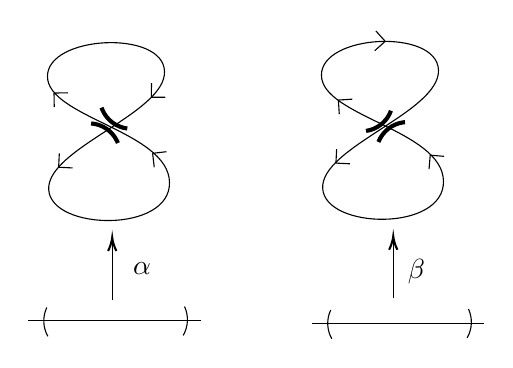
\begin{tikzpicture}[x=0.45pt,y=0.45pt,yscale=-1,xscale=1]
%uncomment if require: \path (0,300); %set diagram left start at 0, and has height of 300

%Shape: Polygon Curved [id:ds7853679117564631] 
\draw   (260.08,40.66) .. controls (259,7) and (166.08,11.66) .. (166.08,44.66) .. controls (166.08,77.66) and (263.08,88.66) .. (264.08,129.66) .. controls (265.08,170.66) and (169.08,168.66) .. (167.08,135.66) .. controls (165.08,102.66) and (261.16,74.32) .. (260.08,40.66) -- cycle ;
%Shape: Polygon Curved [id:ds21040248947928464] 
\draw   (480.08,39.66) .. controls (479,6) and (386.08,10.66) .. (386.08,43.66) .. controls (386.08,76.66) and (483.08,87.66) .. (484.08,128.66) .. controls (485.08,169.66) and (389.08,167.66) .. (387.08,134.66) .. controls (385.08,101.66) and (481.16,73.32) .. (480.08,39.66) -- cycle ;
%Straight Lines [id:da31136821522685154] 
\draw    (150.64,241) -- (289,241) ;
%Shape: Arc [id:dp7840308514297909] 
\draw  [draw opacity=0] (166.38,253.39) .. controls (162.47,246.45) and (161.96,237.83) .. (165.55,230.26) -- (188.3,241.02) -- cycle ; \draw   (166.38,253.39) .. controls (162.47,246.45) and (161.96,237.83) .. (165.55,230.26) ;  
%Shape: Arc [id:dp9158778700317947] 
\draw  [draw opacity=0] (276.17,229.51) .. controls (279.49,236.75) and (279.29,245.38) .. (275.08,252.63) -- (253.3,240.02) -- cycle ; \draw   (276.17,229.51) .. controls (279.49,236.75) and (279.29,245.38) .. (275.08,252.63) ;  
%Straight Lines [id:da2311186184965086] 
\draw    (378.64,243) -- (517,243) ;
%Shape: Arc [id:dp24229069158197247] 
\draw  [draw opacity=0] (394.38,255.39) .. controls (390.47,248.45) and (389.96,239.83) .. (393.55,232.26) -- (416.3,243.02) -- cycle ; \draw   (394.38,255.39) .. controls (390.47,248.45) and (389.96,239.83) .. (393.55,232.26) ;  
%Shape: Arc [id:dp5426990463202246] 
\draw  [draw opacity=0] (504.17,231.51) .. controls (507.49,238.75) and (507.29,247.38) .. (503.08,254.63) -- (481.3,242.02) -- cycle ; \draw   (504.17,231.51) .. controls (507.49,238.75) and (507.29,247.38) .. (503.08,254.63) ;  
%Straight Lines [id:da5214166100333797] 
\draw    (218.08,223.94) -- (218.08,175.94) ;
\draw [shift={(218.08,173.94)}, rotate = 90] [color={rgb, 255:red, 0; green, 0; blue, 0 }  ][line width=0.75]    (10.93,-3.29) .. controls (6.95,-1.4) and (3.31,-0.3) .. (0,0) .. controls (3.31,0.3) and (6.95,1.4) .. (10.93,3.29)   ;
%Straight Lines [id:da1334492905869309] 
\draw    (443.75,222.94) -- (443.75,174.94) ;
\draw [shift={(443.75,172.94)}, rotate = 90] [color={rgb, 255:red, 0; green, 0; blue, 0 }  ][line width=0.75]    (10.93,-3.29) .. controls (6.95,-1.4) and (3.31,-0.3) .. (0,0) .. controls (3.31,0.3) and (6.95,1.4) .. (10.93,3.29)   ;
%Shape: Arc [id:dp950877935154441] 
\draw  [draw opacity=0][line width=1.5]  (201.16,82.45) .. controls (209.8,83.1) and (217.88,88.2) .. (221.94,96.56) .. controls (222.19,97.09) and (222.43,97.62) .. (222.65,98.16) -- (199.3,107.56) -- cycle ; \draw  [line width=1.5]  (201.16,82.45) .. controls (209.8,83.1) and (217.88,88.2) .. (221.94,96.56) .. controls (222.19,97.09) and (222.43,97.62) .. (222.65,98.16) ;  
%Shape: Arc [id:dp7323600781109969] 
\draw  [draw opacity=0][line width=1.5]  (230.15,86.53) .. controls (221.55,85.44) and (213.75,79.93) .. (210.13,71.37) .. controls (209.9,70.83) and (209.69,70.29) .. (209.5,69.74) -- (233.3,61.56) -- cycle ; \draw  [line width=1.5]  (230.15,86.53) .. controls (221.55,85.44) and (213.75,79.93) .. (210.13,71.37) .. controls (209.9,70.83) and (209.69,70.29) .. (209.5,69.74) ;  
%Shape: Arc [id:dp6625974211686132] 
\draw  [draw opacity=0][line width=1.5]  (441.92,72.23) .. controls (439.26,79.48) and (433.3,85.41) .. (425.31,87.73) .. controls (424.18,88.05) and (423.04,88.3) .. (421.91,88.47) -- (418.3,63.56) -- cycle ; \draw  [line width=1.5]  (441.92,72.23) .. controls (439.26,79.48) and (433.3,85.41) .. (425.31,87.73) .. controls (424.18,88.05) and (423.04,88.3) .. (421.91,88.47) ;  
%Shape: Arc [id:dp6178754559947754] 
\draw  [draw opacity=0][line width=1.5]  (431.85,97.36) .. controls (435.01,89.29) and (442.25,83.06) .. (451.44,81.64) .. controls (452.02,81.55) and (452.59,81.48) .. (453.17,81.43) -- (455.3,106.51) -- cycle ; \draw  [line width=1.5]  (431.85,97.36) .. controls (435.01,89.29) and (442.25,83.06) .. (451.44,81.64) .. controls (452.02,81.55) and (452.59,81.48) .. (453.17,81.43) ;  
%Straight Lines [id:da30503229166267887] 
\draw    (175.06,117.63) -- (175.61,106.42) ;
%Straight Lines [id:da9072356484002699] 
\draw    (175.06,117.63) -- (186.27,118.19) ;
%Straight Lines [id:da8384067918800369] 
\draw    (171.34,58.04) -- (182.57,57.85) ;
%Straight Lines [id:da7491709487819667] 
\draw    (171.34,58.04) -- (171.53,69.26) ;
%Straight Lines [id:da5341643742741014] 
\draw    (250.51,106.47) -- (261.66,105.14) ;
%Straight Lines [id:da7507731400759992] 
\draw    (250.51,106.47) -- (251.83,117.62) ;
%Straight Lines [id:da1660661524695084] 
\draw    (249.54,61.41) -- (249.6,50.18) ;
%Straight Lines [id:da3896507949154593] 
\draw    (249.54,61.41) -- (260.77,61.47) ;
%Straight Lines [id:da33709428577659173] 
\draw    (399.68,63.68) -- (410.89,62.96) ;
%Straight Lines [id:da6705414242377215] 
\draw    (399.68,63.68) -- (400.41,74.89) ;
%Straight Lines [id:da30697195840442015] 
\draw    (437.3,16.52) -- (428.93,24.01) ;
%Straight Lines [id:da10060355107370467] 
\draw    (437.3,16.52) -- (429.81,8.16) ;
%Straight Lines [id:da05037827226146252] 
\draw    (397.72,114.3) -- (398.29,103.08) ;
%Straight Lines [id:da44877972781748143] 
\draw    (397.72,114.3) -- (408.93,114.87) ;
%Straight Lines [id:da4798808410915898] 
\draw    (473.44,107.94) -- (484.63,108.88) ;
%Straight Lines [id:da08236318210020843] 
\draw    (473.44,107.94) -- (472.49,119.13) ;

% Text Node
\draw (232.67,192.07) node [anchor=north west][inner sep=0.75pt]    {$\alpha $};
% Text Node
\draw (453.33,189.4) node [anchor=north west][inner sep=0.75pt]    {$\beta $};


\end{tikzpicture}

\caption{Curvas regulares sin reparametrización}
\label{fig:norepar}
\end{figure}
El difeomorfismo $\phi$ no puede anularse, pues eso implicaría que existe un punto en el que $\beta'$ se anula, lo cual es imposible para una curva regular parametrizada. Por lo que si $\phi>0$ le llamaremos reparametrización positiva y si $\phi<0$ será una reparametrización negativa. Si existe una reparametrización de una curva en otra entonces diremos que estas curvas parametrizadas regulares son equivalentes. \\ Una observación importante es la siguiente: Dos curvas parametrizadas regulares pueden tener la misma imagen sin que exista una una reparametrización de una en otra, por ejemplo consideremos las curvas regulares de la Figura \ref{fig:norepar}, no existe difeomorfismo suave tal que $\alpha=\beta\circ\phi$. Si desea darse una prueba de esto se recomiendan las siguientes expresiones para dichas curvas:

\begin{align*}
    \alpha(t)&=\left(\dfrac{\sin(t)}{1+\sin^2(t)},\dfrac{\sin(t)\cos(t)}{1+\sin^2(t)}\right)\\
    \beta(t)&=\left(\dfrac{-\sin(t)}{1+\sin^2(t)},\dfrac{\sin(t)\cos(t)}{1+\sin^2(t)}\right)
\end{align*}
Ambas con domino $(0,2\pi)$. Resulta que un buen objetivo es tratar de estudiar las propiedades que se preservan bajo reparametrizaciones, una de ellas es la longitud de arco de una curva:
\begin{definition}
    Sea $\alpha:I\subset \mathbb{R}\to \mathbb{R}^n$ curva parametrizada regular y $[a,b]\subset I$ un intervalo compacto. \textbf{La longitud de arco} de $\alpha([a,b])$ es el número real
    \begin{align*}
        \ell(\alpha;[a,b])=\int_a^b|\alpha'(t)|dt
    \end{align*}
\end{definition}
De esta definición podemos obtener el siguiente resultado:
\begin{proposition}
    Si $\alpha:I\subset\mathbb{R}\to \mathbb{R}^n$ es una curva parametrizada regular y $\beta=\alpha\circ\phi$. $J\subset \mathbb{R}\to\mathbb{R}^n$ una reparametrización, entonces
    \begin{align*}
        \ell(\beta;[c,d])=\ell(\alpha;\phi([c,d]))
    \end{align*}
\end{proposition}
Una reparamentrización importante es la siguiente
\begin{definition}
    Sea $\alpha:I\subset\mathbb{R}\to\mathbb{R}^n$ una curva regular parametrizada, dicha curva es dicha \textbf{parametrizada por longitud de arco} cuando $|\alpha'(t)|=1$ para todo $t\in I$.
\end{definition}
Un dato importante sobre estas reparametrizaciones es que para toda curva regular parametrizada en $\mathbb{R}^n$ existe una parametrización por longitud de arco. Notemos lo siguiente, si $t_0\in I$, entonces podemos definir
\begin{align*}
    s(t)=\int_{t_0}^t|\alpha'(\xi)|d\xi
\end{align*}
Por el teorema fundamental del cálculo $s'(t)=|\alpha'(t)|$ y por ser $\alpha$ regular parametrizada se tiene $|\alpha'(t)|>0$, por lo que, por el teorema de la función inversa, existe un difeomorfismo $f$ tal que $t=f(s(t))$ y podemos escribir $t(s)=f(s)$ con esto notemos que, si
\begin{align*}
   \beta(s)=\alpha(f(s)) 
\end{align*}
tendremos
\begin{align}
    \beta'(s)=\alpha'(f(s))f'(s) \label{eq:funinversa}
\end{align}
por otro lado, podemos calcular la derivada de una inversa de la siguiente forma
\begin{align*}
    f(s(t))&=t\\
    f'(s(t))s'(t)&=1\\
    f'(s(t))=\dfrac{1}{s'(t)}&=\dfrac{1}{|\alpha'(t)|}
\end{align*}
por lo que si sustituimos en \ref{eq:funinversa} y tomamos norma se tiene que
\begin{align*}
    |\beta'(s)|&=|\alpha'(f(s))f'(s)|\\
    &=\left|\alpha'(f(s))\right|\dfrac{1}{|\alpha'(f(s))|}\\
    &=1.
\end{align*}
Por lo que la reparametrización $\beta=\alpha\circ f$, verifica ser una parametrización por longitud de arco.\\

Con esta teoría desarrollada para curvas en general, nos reduciremos al caso en el que $n=2$, de ahora en adelante, es decir, solamente \textit{curvas planas}.\footnote{De manera más general, una curva plana es una curva regular parametrizada $\alpha:I\subset\mathbb{R}\to \mathbb{R}^3$ para la cual existe un plano $P$ en $\mathbb{R}^3$ tal que $\alpha(I)\subset P$, sin embargo aquí nos fijaremos en las curvas planas contenidas en $\mathbb{R}^2$.} Ahora, si hacemos uso del hecho de que toda curva puede ser reparametrizada por longitud de arco, no importa si solo nos limitamos a usar curvas parametrizadas por longitud de arco. Usaremos esto para definir los siguientes vectores asociados a una curva
\begin{definition}
    Sea $\alpha:I\subset\mathbb{R}\to \mathbb{R}^2$ una curva regular parametrizada, parametrizada por longitud de arco 
    \begin{enumerate}
        \item El vector $T(s)=\alpha'(s)$, es conocido como el \textbf{vector tangente unitario}.
        \item Si $J$ se define como una rotación de $\pi/2$ en sentido antihorario, es decir
        \begin{align*}
    J:\mathbb{R}^2&\to \mathbb{R}^2\\
    (x,y)&\mapsto (-y,x).
\end{align*}
se define $N(s)=J\alpha'(s)$ como el \textbf{vector normal unitario}.
    \end{enumerate}
\end{definition}
Algunas de las propiedades de estos vectores son:
\begin{proposition}\label{propprodtn}
    Si $T(s)$ y $N(s)$ son los vectores tangente unitario y normal unitario de una curva regular\footnote{El termino correcto sería curva regular parametrizada, parametrizada por longitud de arco, pero desde este punto omitiremos esta parte del nombre.} parametrizada por longitud de arco entonces
    \begin{enumerate}
        \item[$i)$] $\langle T'(s),T(s)\rangle=0$.
        \item[$ii)$] $\langle N'(s),N(s)\rangle=0$.
        \item[$iii)$] $\langle N'(s),T(s)\rangle=-\langle N(s),T'(s)\rangle$.
    \end{enumerate}
\end{proposition}
De estas propiedades y usando el hecho de que estamos en $\mathbb{R}^2$ podemos concluir que $T'(s)\parallel N(s)$ y $N'(s) \parallel T(s)$.
\section{Curvatura con signo}
Con la misma notación que hemos adoptado dentro del texto, tengamos en cuenta lo siguiente: Al ser $T(s)$ y $N(s)$ dos vectores no nulos y ortogonales, forman una base para $\mathbb{R}^2$ visto como espacio vectorial. Por lo que si expresamos los vectores $T'(s)$ y $N'(s)$ como combinación lineal de $T$ y $N$:
\begin{align*}
    T'(s)&=aT(s)+bN(s)\\
    N'(s)&=cT(s)+dN(s).
\end{align*}
Al aplicar producto internos con los vectores adecuados adecuados y por \ref{propprodtn}, se se sigue que $-b=c$ y $a=d=0$. Por su unicidad, pues son coeficientes de estos vectores, tiene sentido darle un nombre a este número $b$. 
\begin{definition}
    Sea $\alpha:I\subset \mathbb{R}\to \mathbb{R}^2$ una curva plana regular, parametrizada por longitud de arco. La \textbf{curvatura con signo} de $\alpha$ en $s\in I$ es el único número $k$ tal que $T'(s)=k(s)N(s)$, es decir 
\begin{align*}
    k(s):=\langle T'(s), N(s)\rangle.
\end{align*}
\end{definition}
Esto es algo que no definiremos en curvas en $\mathbb{R}^3$ (aunque puede hacerse) y es que las curvas en $\mathbb{R}^2$ tienen signo y este cambia bajo reparametrizaciones negativas. Pero ¿qué significa este número realmente? Podemos encontrar una interpretación del signo de la curvatura en \cite[p.~22]{do2016differential} basada en la orientación de las base $\{e_1,e_2\}$\footnote{También es posible asignarle un signo a la curvatura de una curva en $\mathbb{R}^3$ pero se debe usar la orientación de $\{e_1,e_2,e_3\}$, consultar el apéndice A.}. 
\begin{definition}
    Si  $T(s),N(s)$ son definidos como con anterioridad, a la base $\{T(s),N(s)\}$ se le conoce como \textbf{diedro de Frenet}.
\end{definition}
Y usualmente se escribe como el siguiente sistema de ecuaciones diferenciales:
\begin{align}
\begin{bmatrix}
    T(s)\\
    N(s)
\end{bmatrix}
'
=
\begin{bmatrix}
    0_2 & k I_2\\
    -k I_2 & 0_2
\end{bmatrix}
\begin{bmatrix}
    T(s)\\
    N(s)
\end{bmatrix}
\label{sistema2dfrenet}
\end{align}
El sistema \ref{sistema2dfrenet}, nos da una pista de que dada una función suave $k=k(s)$, podemos encontrar un vector tangente y un vector normal y eso reconstruye de alguna manera la curva regular de la cual $T$ y $N$ son los vectores tangente y normal. Esta es una posibilidad pero presentaremos una alternativa usando funciones angulares en lugar de una prueba que involucre soluciones a ecuaciones diferenciales, pues para ello hay que usar resultados de existencia y unicidad. Sea $I\subset \mathbb{R}$ un intervalo abierto y $\mathbb{S}^1=\{p\in \mathbb{R}^2|\hspace{0.1 cm} |p|=1\}\subset \mathbb{R}^2$ el círculo unitario de radio $1$ centrado en el origen. Los puntos de $\mathbb{S}^1$ son de la forma $p=(\cos\theta,\sin\theta)$ para algún $\theta\in \mathbb{R}$.
\begin{definition}
    Sea $\mathbb{\gamma}:I\to\mathbb{S}^1$ una función suave. Una \textbf{función angular suave} para $\gamma$ es una  función suave $\theta:I\to\mathbb{R}$ tal que
    \begin{align*}
        \gamma(t)=(\cos\theta(t), \sin\theta(t)) \quad \text{para todo }t\in I.
    \end{align*}
\end{definition}
Si se considera la aplicación $E:u\in \mathbb{R}\mapsto (\cos u, \sin u)\in \mathbb{S}^1$, también llamada \textbf{aplicación exponencial}. Se puede resumir la definición previa por medio del siguiente diagrama conmutativo:
\begin{center}
 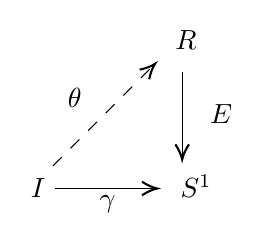
\begin{tikzpicture}[x=0.5pt,y=0.5pt,yscale=-1,xscale=1]
%uncomment if require: \path (0,300); %set diagram left start at 0, and has height of 300

%Straight Lines [id:da3628861471491769] 
\draw  [dash pattern={on 4.5pt off 4.5pt}]  (264.24,170.75) -- (336.66,98.33) ;
\draw [shift={(338.07,96.91)}, rotate = 135] [color={rgb, 255:red, 0; green, 0; blue, 0 }  ][line width=0.75]    (10.93,-4.9) .. controls (6.95,-2.3) and (3.31,-0.67) .. (0,0) .. controls (3.31,0.67) and (6.95,2.3) .. (10.93,4.9)   ;
%Straight Lines [id:da17201270472498598] 
\draw    (265.72,187.06) -- (337.56,187.06) ;
\draw [shift={(339.56,187.06)}, rotate = 180] [color={rgb, 255:red, 0; green, 0; blue, 0 }  ][line width=0.75]    (10.93,-4.9) .. controls (6.95,-2.3) and (3.31,-0.67) .. (0,0) .. controls (3.31,0.67) and (6.95,2.3) .. (10.93,4.9)   ;
%Straight Lines [id:da7802681839004739] 
\draw    (357.64,102.55) -- (357.64,164.11) ;
\draw [shift={(357.64,166.11)}, rotate = 270] [color={rgb, 255:red, 0; green, 0; blue, 0 }  ][line width=0.75]    (10.93,-4.9) .. controls (6.95,-2.3) and (3.31,-0.67) .. (0,0) .. controls (3.31,0.67) and (6.95,2.3) .. (10.93,4.9)   ;

% Text Node
\draw (246.38,177.97) node [anchor=north west][inner sep=0.75pt]    {$I$};
% Text Node
\draw (273.07,112.74) node [anchor=north west][inner sep=0.75pt]    {$\theta $};
% Text Node
\draw (350.88,71.23) node [anchor=north west][inner sep=0.75pt]    {$\mathbb{R}$};
% Text Node
\draw (354.57,175.49) node [anchor=north west][inner sep=0.75pt]    {$\mathbb{S}^{1}$};
% Text Node
\draw (376,124.4) node [anchor=north west][inner sep=0.75pt]    {$E$};
% Text Node
\draw (296,190.4) node [anchor=north west][inner sep=0.75pt]    {$\gamma $};
\end{tikzpicture}
\end{center}
(El significado del diagrama es el siguiente: $\theta$ es una función angular para $\gamma$
 cuando  $\gamma=E\circ \theta$ ).

Como $\cos$ y $\sin$ son funciones periódicas con período $2\pi$, las funciones angulares no son únicas.
Sin embargo, esta es la única indeterminación:
\begin{lemma}
    Si $\theta_1$ y $\theta_2$ dos dos funciones angulares suaves para una función suave $\gamma:I\to \mathbb{S}^1$, entonces existe un entero $k\in\mathbb{Z}$ tal que
    \begin{align*}
        \theta_2(t)-\theta_1(t)=2\pi k\quad\text{para todo }t\in I.
    \end{align*}
\end{lemma}
\textit{Demostración.} La diferencia $\theta_2-\theta_1$ y una función suave (en particular, continua)
tomando valores en el conjunto discreto formado por números enteros múltiplos de $2$. como $I$ es un intervalo (en particular, conexo), la diferencia $\theta_2-\theta_1$ es constante. \hfill $\blacksquare$

En particular, la derivada de $\theta$ está determinada únicamente por la función $\gamma$:
\begin{lemma}
    Sea $\gamma=(x,y):I\to \mathbb{S}^1$ una función suave. Si $\theta:I\to \mathbb{R}$ es una función angular suave para $\gamma$, entonces
    \begin{align*}
    \theta'=-yx'+xy' \text{ en }I.
\end{align*}
\end{lemma}
\textit{Demostración.} Escribiendo $\gamma=(x,y)$ en coordenadas euclideanas, se tendrá que $x^2(t)+y^2(t)=1$ y por la regla de la cadena se tiene
\begin{align*}
    (x,y)&=(\cos \theta, \sin\theta)\\ (x',y')&=(-\theta'\sin\theta,\theta'\cos\theta)=\theta'(-y,x).
\end{align*}
En particular
\begin{align*}
    -yx'+xy'&=-y(-y\theta')+x(x\theta')\\
    &=(x^2+y^2)\theta'=\theta'.
\end{align*}
Esta observación sugiere cómo construir funciones angulares. De hecho, podemos demostrar
que
\begin{proposition}
    Toda función suave $\gamma:I\to\mathbb{S}^1$ admite una función angular suave.
    \label{existfangular}
\end{proposition}
\textit{Demostración.} Escribimos $\gamma=(x,y)$ en coordenadas Euclideanas. Si escojemos algún $t_0\in I$, y algún $t_0\in \mathbb{R}$ tal que $\gamma(t_0)=(\cos\theta_0,\sin\theta_0)$. Entonces, definimos una función $\theta:I\to\mathbb{R}$ de la siguiente forma
\begin{align*}
    \theta(t):=\theta_0+\int_{t_0}^t(-y(u)x'(u)+x(u)y'(u))du\\ \text{ para todo }t\in I.
\end{align*}
Como $\gamma$ es suave en $I$, entonces $\theta$ lo es también en $I$. Sea $\hat{\gamma}:I\to\mathbb{R}^2$ dada por 
\begin{align*}
    \hat{\gamma}=(\cos \theta(t), \sin\theta(t)) \text{ para todo }t\in I.
\end{align*}
Para concluir la demostración, basta mostrar que $\gamma=\hat{\gamma}$, pues en este caso la función 
$\theta$, será nuestra función angular suave para $\gamma$. 

Ahora, en virtud de la definición de $\theta$, se define  $\hat{\gamma}(t_0)=(\cos\theta_0, \sin\theta_0)=\gamma(t_0)$ y
\begin{align*}
    \hat{\gamma}'=\theta'(-\sin\theta,\cos\theta)=(-yx'+xy')J\hat{\gamma}.
\end{align*}
Por otro lado, observe que $|\gamma|=x^2+y^2=1$ implica $\langle\gamma,\gamma'\rangle=xx'+yy'=0$. Siendo $\gamma$ ortogonal a $\gamma'$ y un múltiplo de $J\gamma$. Un cálculo directo usando estas identidades muestra lo siguiente
\begin{align*}
    \gamma'=(-yx'+xy')J\gamma.
\end{align*}
Usando estas fórmulas para las derivadas de $\gamma$ y $\hat{\gamma}$ calculadas con anterioridad nos ayuda a concluir que:
\begin{align*}
    \dfrac{1}{2}(|\gamma-\gamma'|^2)'&=\langle\gamma-\hat{\gamma}, \gamma'-\hat{\gamma}'\rangle\\
    &=(-yx'+xy')\langle\gamma-\hat{\gamma}, J\gamma-J\hat{\gamma}\rangle\\
    &=(-yx'+xy')\langle\gamma-\hat{\gamma}, J(\gamma-\hat{\gamma})\rangle\\
    &=0
\end{align*}
idénticamente en el intervalo $I$. Por tanto $|\gamma-\hat{\gamma}|$ es una función constante en $I$. Como $\gamma(t_0)=\hat{\gamma}(t_0)$, tenemos que $\gamma\equiv\hat{\gamma}$.\hfill $\blacksquare$ 

\textbf{Observación:} El vector unitario tangente de una curva plana parametrizada por la longitud
de arco $\alpha=(x, y): I \to \mathbb{R}^2$, define una función suave $T:=\alpha' = (x', y') : I \to \mathbb{S}^1$, la cual admite una función angular suave, en virtud de la Proposición \ref{existfangular}. Este hecho se puede utilizar argumentar que la curvatura con signo, no es más que la derivada de la función angular del vector tangente unitario $T$. 

La definición de estas funciones angulares nos permite dar una demostración del teorema fundamental de curvas planas. El cual es una observación que se hizo en $\ref{sistema2dfrenet}$.
\begin{theorem}[\tiny Teorema fundamental de curvas planas] Sea $k:I\subset \mathbb{R}\to\mathbb{R}$ es una función suave entonces existe una curva regular parametrizada parametrizada por longitud de arco $\alpha:I\subset \mathbb{R}\to\mathbb{R}^2$ cuya curvatura en $s\in I$ es $k(s)$ para todo $s\in I$. Además, si $\alpha_1,\alpha_2:I\subset \mathbb{R}\to\mathbb{R}^2$ son curvas parametrizadas por longitud de arco con una misma función curvatura con signo en $I$, entonces existe un movimiento rígido $M:\mathbb{R}^2\to\mathbb{R}^2$ tal que $\alpha_2=M\circ \alpha_1$. 
    
\end{theorem}
Para una prueba de este teorema usando funciones angulares ver \cite[p.~13]{montiel2009curves}. Posteriormente mostraremos un resultado muy parecido a este pero con curvas que viven en otra variedad (para más detalles sobre el concepto de variedad consúltese el Apéndice B) de dimensión $2$, en concreto daremos un teorema fundamental de curvas en $\mathbb{S}^2$ y como sería de esperarse, también en esta variedad las curvas también están caracterizadas únicamente por una función suave.

Un resultado conocido del cual invitamos al lector a intentar dar una demostración como ejercicio, es el siguiente:
\begin{proposition}
    Sea $\alpha:I\subset \mathbb{R}\to \mathbb{R}^2$ una curva parametrizada regular, con curvatura constante $k_0\neq 0$, entonces la imagen de $\alpha$ está enteramente contenida en un círculo.
\end{proposition}
Finalmente y para fines prácticos para calcular curvaturas de curvas planas en $\mathbb{R}^2$, podemos usar la siguiente expresión:
\begin{proposition}
Si $\alpha:I\subset \mathbb{R}$ es una curva regular parametrizada (no necesariamente por longitud de arco) entonces su curvatura con signo para una parametrización $\alpha$ denotada por $k_\alpha$ en un punto $t\in I$ viene dada por
\begin{align*}
    k_\alpha(t)=\dfrac{1}{|\alpha'(t)|^3}\det(\alpha'(t), \alpha''(t)).
\end{align*}   
Notese que cuando $\alpha$ es una parametrización por longitud de arco se tiene que
\begin{align*}
    k(s)=k_\alpha(s)=\det(T(s), T'(s))
\end{align*}
\end{proposition}
\textit{Demostración.} 
Si $\beta$ es la reparametrización de $\alpha$ por longitud de arco, y $t=f(s)$ se tiene que
\begin{align*}
    f'(s)=\dfrac{1}{|\alpha'(f(s))|},
\end{align*}
además
\begin{align}
    \beta'(s)&=\alpha'(f(s))f'(s)\nonumber\\
    \beta''(s)&=\alpha''(f(s))[f'(s)]^2+\alpha'(f(s))f''(s)\label{ref:difeolongitudarco}
\end{align}
luego
\begin{align*}
    k_\alpha(t)&=k_\beta(f^{-1}(t))\\
               &=k_\beta(s)\\
               &=k(s)\\
               &=\langle\beta''(s),J\beta'(s)\rangle
\end{align*}
una identidad que puede ser probada expandiendo por componentes es $\langle v,Jw\rangle=\det(v,w)$. Por lo que tendremos por las relaciones \ref{ref:difeolongitudarco} y usando la linealidad por componentes del determinante
\begin{align*}
    k_\alpha(f(s))&= \left( f'(s)\right)^3\det(\alpha'(f(s)), \alpha''(f(s)))
\end{align*}
y usando que $t=f(s)$ obtendremos la fórmula buscada. \hfill $\blacksquare$
\section{Ejercicios}

%%%%%%%%%%%%%%%%%%%%%%%%%%%%%%%%%%%%%%%%%%%%%%%%%%%%%%%%%%%%%%%%%%%%%
\chapter{Una desigualdad geométrica}
Dentro del contexto de la geometría diferencial de curvas planas, el desarrollo de algunos resultados deriva de las relaciones entre curvas cerradas y el área encerrada por ellas. Sin embargo, aunque varios de estos conceptos parezcan simples y algunas de las proposiciones parezcan triviales, definirlos de manera adecuada puede ser poco intuitivo. Por ello dedicaremos un espacio específico a la teoría de curvas cerradas concluyendo con una desigualdad muy famosa que motiva el desarrollo de problemas en más dimensiones o problemas con más condiciones, pero sin salir de $\mathbb{R}^2$.
\section{Curvas Cerradas}
La primera definición, es simple pero fundamental. 
\begin{definition}
    Una \textbf{curva regular parametrizada cerrada} es una aplicación $\alpha:[a,b]\subset \mathbb{R}\to\mathbb{R}^2$, con $[a,b]$ compacto, que es suave, verifica $\alpha'(t)\neq 0$ para todo $t\in [a,b]$ y es tal que $\alpha(a)=\alpha(b)$,  $\alpha'(a)=\alpha'(b)$, $\alpha''(a)=\alpha''(b),\ldots$ etc. Es decir, todas sus derivadas coinciden en $a$ y $b$. 
\end{definition}
Tomando en cuenta que 
\begin{align*}
   \alpha'(a)&=\lim_{t\to 0^+}\dfrac{\alpha(a+t)-\alpha(a)}{t}. \\
   \alpha'(b)&=\lim_{t\to 0^-}\dfrac{\alpha(b+t)-\alpha(b)}{t}. 
\end{align*}
Siendo esta una definición de la cual deriva la siguiente:
\begin{definition}
    Una curva regular parametrizada cerrada $\alpha:[a,b]\to\mathbb{R}^2$, es llamada \textbf{simple} cuando $\left.\alpha\right|_{[a,b)}$ es inyectiva.
\end{definition}
Ejemplos de esto en la \ref{fig:curvascerradas}.
\begin{figure}[h]
    \centering
    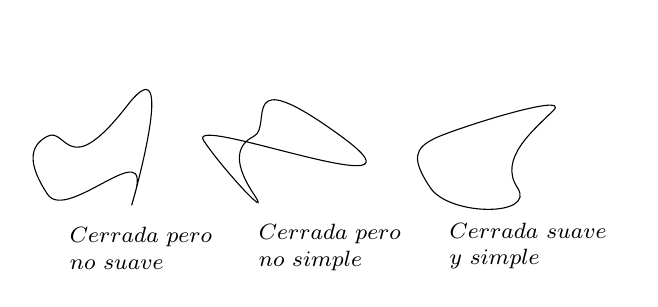
\begin{tikzpicture}[x=0.35pt,y=0.35pt,yscale=-1,xscale=1]
%uncomment if require: \path (0,300); %set diagram left start at 0, and has height of 300

%Shape: Polygon Curved [id:ds9446676613476299] 
\draw   (81,82) .. controls (101,72) and (101.08,130.5) .. (163.08,50.5) .. controls (225.08,-29.5) and (152.08,206.5) .. (171,142) .. controls (189.92,77.5) and (101,172) .. (81,142) .. controls (61,112) and (61,92) .. (81,82) -- cycle ;
%Shape: Polygon Curved [id:ds11442323004809563] 
\draw   (294,82) .. controls (314,72) and (274.92,2.5) .. (384,82) .. controls (493.08,161.5) and (222.08,56.5) .. (242.08,86.5) .. controls (262.08,116.5) and (314,172) .. (294,142) .. controls (274,112) and (274,92) .. (294,82) -- cycle ;
%Shape: Polygon Curved [id:ds4789651120255243] 
\draw   (480.08,84.5) .. controls (500.08,74.5) and (623.08,35.5) .. (603.08,55.5) .. controls (583.08,75.5) and (546,105) .. (566,135) .. controls (586,165) and (496,165) .. (476,135) .. controls (456,105) and (460.08,94.5) .. (480.08,84.5) -- cycle ;

% Text Node
\draw (87,170.4) node [anchor=north west][inner sep=0.75pt]  [font=\footnotesize]  {$ \begin{array}{l}
Cerrada\ pero\ \\
no\ suave
\end{array}$};
% Text Node
\draw (282,167.4) node [anchor=north west][inner sep=0.75pt]  [font=\footnotesize]  {$ \begin{array}{l}
Cerrada\ pero\\
no\ simple
\end{array}$};
% Text Node
\draw (479,165.4) node [anchor=north west][inner sep=0.75pt]  [font=\footnotesize]  {$ \begin{array}{l}
Cerrada\ suave\ \\
y\ simple
\end{array}$};
\end{tikzpicture}
    \caption{Tipos de curvas.}
    \label{fig:curvascerradas}
\end{figure}
\\

Estas curvas cerradas simples tienen algunas propiedades topológicas interesantes, una de ellas es que su imagen es homeomorfa a $\mathbb{S}^1$. A estas curvas les pondremos un nombre específico.
\begin{definition}
    \textbf{Una curva de Jordan} en $\mathbb{R}^n$ es un conjunto $C$ que es imágen de una aplicación contínua e inyectiva $\gamma:\mathbb{S}^1\to\mathbb{R}^n$.
\end{definition}
Siendo estos, algunos resultados sobre curvas cerradas.
\begin{theorem}[Teorema de Jordan]
   Sea $C\subset \mathbb{R}^2$ es una curva de Jordan, entonces
   \begin{itemize}
       \item[i)] $\mathbb{R}^2-C$ tiene dos componentes conexas no vacías.
       \item[ii)] Una de estas componentes es no acotada y la otra si es acotada. 
       \item[iii)] La frontera de ambas componentes es $C$. 
   \end{itemize}
\end{theorem}
Siendo este teorema es objeto de estudio en topología, así que no nos centraremos en dar una prueba en este documento. 

Una extensión poco conocida de este teorema es la siguiente, de la cual podemos encontrar una prueba elemental en \cite{JS}.
\begin{theorem}[Jordan-Schönflies] 
    Una curva simple cerrada $C$ en un plano $E$ separa $E$ en dos regiones. Y existe un auto-homeomorfismo de $E$ a $E$ tal que este mapea $C$ en un círculo contenido en $E$.
\end{theorem}
Bien definidas estas regiones, podremos definir el área, dada una curva regular cerrada. Si $\alpha:[a,b]\to \mathbb{R}^2$ curva regular cerrada y simple, parametrizada por longitud de arco $\Omega=$región compacta delimitada por $\alpha([a,b])$. Donde $\alpha$ está orientada de forma que el vector normal unitario $N(s)$, apunta a $\Omega$ para todo $s\in I$, vistas en \ref{fig:areayorientasion}.
\begin{figure}[h]
    \begin{center}
  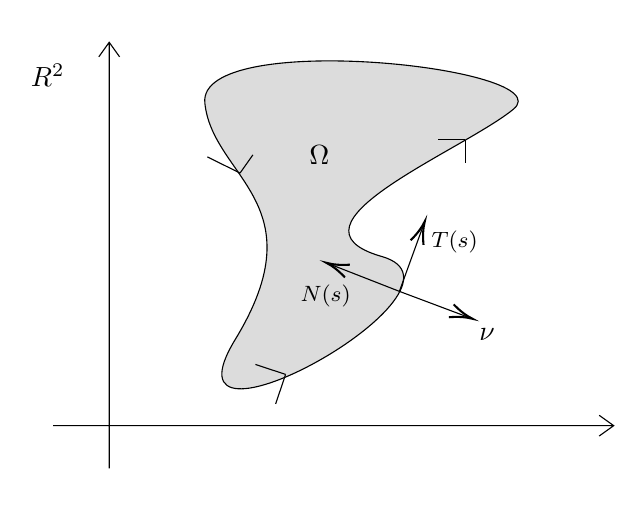
\begin{tikzpicture}[x=0.75pt,y=0.75pt,yscale=-1,xscale=1]
%uncomment if require: \path (0,300); %set diagram left start at 0, and has height of 300

%Shape: Axis 2D [id:dp8770080386298975] 
\draw  (178,231.7) -- (448.08,231.7)(205.01,47) -- (205.01,252.22) (441.08,226.7) -- (448.08,231.7) -- (441.08,236.7) (200.01,54) -- (205.01,47) -- (210.01,54)  ;
%Shape: Polygon Curved [id:ds08136601121953912] 
\draw  [fill={rgb, 255:red, 155; green, 155; blue, 155 }  ,fill opacity=0.35 ] (251.09,76.22) .. controls (247.43,40.22) and (424.14,59.22) .. (399.77,79.22) .. controls (375.4,99.22) and (283.99,135.22) .. (336.4,150.22) .. controls (388.8,165.22) and (225.5,256.22) .. (265.71,190.22) .. controls (305.93,124.22) and (254.75,112.22) .. (251.09,76.22) -- cycle ;
%Straight Lines [id:da5953818299203686] 
\draw    (344.83,167) -- (356.4,135.1) ;
\draw [shift={(357.08,133.22)}, rotate = 109.93] [color={rgb, 255:red, 0; green, 0; blue, 0 }  ][line width=0.75]    (10.93,-3.29) .. controls (6.95,-1.4) and (3.31,-0.3) .. (0,0) .. controls (3.31,0.3) and (6.95,1.4) .. (10.93,3.29)   ;
%Straight Lines [id:da8517959742714176] 
\draw    (344.83,167) -- (311.45,153.95) ;
\draw [shift={(309.59,153.22)}, rotate = 21.35] [color={rgb, 255:red, 0; green, 0; blue, 0 }  ][line width=0.75]    (10.93,-3.29) .. controls (6.95,-1.4) and (3.31,-0.3) .. (0,0) .. controls (3.31,0.3) and (6.95,1.4) .. (10.93,3.29)   ;
%Straight Lines [id:da7681453020700912] 
\draw    (376.52,94) -- (376.52,105.22) ;
%Straight Lines [id:da3106951620466676] 
\draw    (376.52,94) -- (363.21,94) ;
%Straight Lines [id:da2746708084637135] 
\draw    (252.31,102.22) -- (268.05,110) ;
%Straight Lines [id:da8451253105611829] 
\draw    (268.05,110) -- (274.25,101.22) ;
%Straight Lines [id:da5883133213294807] 
\draw    (289.99,207) -- (285.21,221.22) ;
%Straight Lines [id:da026533255731403305] 
\draw    (275.46,202.22) -- (289.99,207) ;
%Straight Lines [id:da508542019439262] 
\draw    (344.83,167) -- (378.21,179.52) ;
\draw [shift={(380.08,180.22)}, rotate = 200.56] [color={rgb, 255:red, 0; green, 0; blue, 0 }  ][line width=0.75]    (10.93,-3.29) .. controls (6.95,-1.4) and (3.31,-0.3) .. (0,0) .. controls (3.31,0.3) and (6.95,1.4) .. (10.93,3.29)   ;

% Text Node
\draw (300.16,95.4) node [anchor=north west][inner sep=0.75pt]    {$\Omega $};
% Text Node
\draw (359.08,136.62) node [anchor=north west][inner sep=0.75pt]  [font=\footnotesize]  {$T( s)$};
% Text Node
\draw (295.93,162.51) node [anchor=north west][inner sep=0.75pt]  [font=\footnotesize]  {$N( s)$};
% Text Node
\draw (166,56.4) node [anchor=north west][inner sep=0.75pt]    {$\mathbb{R}^{2}$};
% Text Node
\draw (382.08,183.62) node [anchor=north west][inner sep=0.75pt]    {$\nu $};


\end{tikzpicture}
    \end{center}
    \caption{Área encerrada por una curva cerrada orientada con sus vectores tangente, normal.}
    \label{fig:areayorientasion}
\end{figure}
\\

Para el cálculo de la longitud, ya tenemos una idea de como hacer la cuenta
\begin{align*}
    \ell(\alpha;[a,b])=\int_a^b|\alpha'(t)|dt=b-a=L.
\end{align*}
Para calcular el área delimitada por $\alpha$ necesitaremos los siguientes resultados
\begin{theorem}[Gauss Green]
    Para todo campo de vectores suave $X:U\subset\mathbb{R}^2\to\mathbb{R}^2$, $U\supset \Omega$.
    \begin{align*}
        \int_\Omega \text{div 
 }X=\int_{\partial \Omega}\langle X,\nu\rangle.
    \end{align*}
    Donde, si $X(x,y)=(a(x,y),b(x,y))$ entonces
    \begin{align*}
    \text{div }X=\nabla \cdot X=\dfrac{\partial a}{\partial x}(x,y)+\dfrac{\partial b}{\partial y}(x,y),
    \end{align*}
    $\nu$ es un vector normal unitario apuntando afuera de la región y además
    \begin{align*}
        \int_{\partial \Omega}\langle X,\nu\rangle= \int_a^b\langle X(\alpha(s)),\nu(\alpha(s))\rangle |\alpha'(s)|ds.
    \end{align*}
\end{theorem}
Un tratamiento más profundidad de este teorema se puede encontrar en \cite{lima1981curso}. 

Usando \textit{Gauss Green} es posible encontrar el área de una región acotada por una curva cerrada $\alpha:[a,b]\to \mathbb{R}^2$, esto de la siguiente forma, si $X(x,y)=(x,y)$ entonces
\begin{align*}
    A(\Omega)&=\int_{\Omega}1\\
            &=\dfrac{1}{2}\int_{\Omega}\text{div }X\\
            &=\dfrac{1}{2}\int_{\partial\Omega}\left\langle X,\nu\right\rangle 
\end{align*}
si $\alpha(s)=(x(s),y(s))$ está parametrizada por longitud de arco tendremos que
\begin{align*}
    T(s)&=\alpha'(s)=(x'(s),y'(s))\\
    N(s)&=(-y'(s),x(s))\\
    \nu(s)&=(y'(s),-x'(s))
\end{align*}
y con esto tendremos 
\begin{align*}
    A(\Omega)=\dfrac{1}{2}\int_{a}^b(x(s)y'(s)-x'(s)y(s))ds.
\end{align*}
siendo esta una expresión estándar para el cálculo de áreas.\\

Y antes de presentar el problema isoperimetrico, mostraremos una desigualdad que surge como una consecuencia de la expansión de Fourier de una función, que nos servirá posteriormente.
\begin{lemma}[Desigualdad de Wirtinger]
   Sea $f:\mathbb{R}\to\mathbb{R}$ es una función suave periódica de periodo $2\pi$ tal que $\int_{0}^{2\pi}f(s)ds=0$, entonces
   \begin{align*}
       \int_{0}^{2\pi}(f'(s))^2ds\geq \int _0^{2\pi}f(s)^2ds
   \end{align*}
\end{lemma}
 La hipótesis sobre el promedio de $f$ en el intervalo $[0,2\pi]$ excluye funciones constantes distintas de cero, pues que incumplen la desigualdad anterior. 
   
Con respecto al producto interno definido como
\begin{align*}
    \langle f,g\rangle_{L^2}=\int_{0}^{2\pi}f(s)g(s)ds .
\end{align*}
Una función periódica suave $f$ de período $2\pi$ tiene media cero en $[0,2\pi]$ si y sólo si $f$ es ortogonal a todas las funciones constantes.


Para demostrar la desigualdad de Wirtinger, usaremos algunas ideas de la teoría de series de Fourier. En su estudio de la ecuación del calor, Joseph Fourier consideró la posibilidad de escribir una función periódica arbitraria como una suma infinita de funciones periódicas elementales:
\begin{align}
    f(s)=\dfrac{a_0}{2}+\sum_{n=1}^{\infty}(a_n\cos(ns)+b_n\sin(ns)).
    \label{eq:expansionfourier}
\end{align}
Motivado por el producto interno definido anteriormente y la expresión (formal) de $f$. Con respecto a la base ortonormal infinita formada por las funciones periódicas elementales, la Los coeficientes de Fourier $a_n$, $b_n$ están definidos por las fórmulas
\begin{align*}
    a_0&=\dfrac{1}{\pi}\int_0^{2\pi}f(s)ds\\
    a_n&=\dfrac{1}{\pi}\int_0^{2\pi}f(s)\cos(ns)ds\\
    b_n&=\dfrac{1}{\pi}\int_0^{2\pi}f(s)\sin(ns)ds
\end{align*}
Y estos coeficientes pueden ser deducidos directamente de \ref{eq:expansionfourier}. Con esto podremos mostrar el \textit{teorema de parseval} el cual nos indica que la siguiente identidad es cierta
\begin{align*}
    \dfrac{1}{\pi}\int_{0}^{2\pi}f(s)^2ds=\dfrac{a_0^2}{2}+\sum_{n=1}^{\infty}(a_n^2+b_n^2).
\end{align*}
Si se desea profundizar un poco en estos resultados, se recomienda la lectura de \cite{stein2011fourier}, pero con la teoría desarrollada hasta ahora podemos mostrar esta la desigualdad.

\textit{Demostración. }Calculamos los coeficientes de Fourier $a_n$, $b_n$ de la función periódica suave $f$ con período $2\pi$ y promedio cero en el intervalo $[0,2\pi]$, y luego los comparamos con los coeficientes de
Fourier $a_n'$ y $b_n'$ de su derivada $f'$, que también es una función suave periódica del mismo periodo. Como $f$ tiene media cero en el intervalo $[0,2\pi]$, tenemos
\begin{align*}
    a_0=\dfrac{1}{\pi}\int_{0}^{2\pi}f(s)ds=0.
\end{align*}
Como $f$ es periódica con periodo $2\pi$, tenemos
\begin{align*}
    a_0':=\dfrac{1}{\pi}\int_{0}^{2\pi}f'(s)ds=\dfrac{1}{\pi}(f(2\pi)-f(0))=0.
\end{align*}
Luego, una integración por partes nos muestra que
\begin{align*}
   a_n'&=\dfrac{1}{\pi}\int_0^{2\pi}f'(s)\cos(ns)ds=nb_n,\\
    b_n'&=\dfrac{1}{\pi}\int_0^{2\pi}f'(s)\sin(ns)ds =-na_n
\end{align*}
y usando la identidad de Parseval obtendremos que
\begin{align*}
    \dfrac{1}{\pi}\int_{0}^{2\pi}(f')^2(s)ds&=\sum_{n=1}^\infty((a_n')^2+(b_n')^2)\\
    &=\sum_{n=1}^{\infty}n^2(a_n^2+b_n^2)\\
    &\geq\sum_{n=1}^{\infty}(a_n^2+b_n^2)\\
    &=\dfrac{1}{\pi}\int_{0}^{2\pi}f^2(s)ds.
\end{align*}
\hfill $\blacksquare$

Ahora bien, con un poco más de esfuerzo podemos mostrar lo mismo, pero para funciones suaves de periodo arbitrario
\begin{theorem}
    Si $f$ es una función continua y con derivada continua en el intervalo $[0,L]$ que verifica $\int_{0}^Lf(s)ds=0$ y $f(0)=f(L)$.  Entonces
    \begin{align*}
        \int_0^L f^2(s)ds\leq \dfrac{L^2}{4\pi^2}\int_0^L f'(s)^2ds
    \end{align*}
\end{theorem}
Siendo este un último lema necesario para la prueba y presentación de una desigualdad fundamental en este capítulo.

Consideremos el siguiente problema de optimización: \textit{Dentro de todas las curvas regulares cerradas y simples que tienen la misma longitud de arco ¿Cuál de ellas delimita la región de mayor área?} La respuesta corta es, el círculo. Para la respuesta larga y la justificación, procederemos a expresar esto en términos de desigualdades algebraicas y formularlo de manera correcta. Si $L$ es la longitud de la curva o el perímetro, y $A$ denota el área, usando las expresiones que conocemos para ambas cantidades tendremos que el cociente $L^2/A$ es invariante bajo dilataciones. Ahora, para un círculo de radio $R$ veamos lo siguiente
\begin{align*}
    \dfrac{L^2}{A}=\dfrac{(2\pi R)^2}{\pi R^2}=\dfrac{4\pi^2 R^2}{\pi R^2}=4\pi.
\end{align*}
Siendo este caso particular, algo que podría parecer una coincidencia sin más pero esconde un resultado aún más profundo.
\begin{theorem}[\footnotesize{Desigualdad Isoperimétrica}]
    Sea $\alpha$ una curva plana parametrizada regular, cerrada con longitud $L$ que delimita una región con área $A$, entonces
    \begin{align*}
        \dfrac{L^2}{A}\geq 4\pi
    \end{align*}
    Teniendo la igualdad si y solo si, la imagen de $\alpha$ es un círculo.
\end{theorem}
Sin pérdida de generalidad asumiremos lo siguiente:
\begin{itemize}
    \item $\alpha$ está parametrizada por longitud de arco. y $\alpha:[0,L]\to\mathbb{R}^2$.
    \item Por la invarianza bajo dilataciones podremos elegir $L=2\pi$. 
    \item Se escoge $\int_{0}^{2\pi} x(s)ds=\int_{0}^{2\pi} y(s)ds=0$.
\end{itemize}
Bajo estas, premisas lo que hay que mostrar es:
\begin{align*}
    A\leq \pi
\end{align*}
Entonces veamos que
\begin{align*}
    A&=\dfrac{1}{2}\int_{0}^{2\pi}(x(s)y'(s)-x'(s)y(s))ds,
\end{align*}
usando la desigualdad AM-GM, tendremos
\begin{align}
    x(s)y'(s)&\leq \dfrac{x^2(s)+(y'(s))^2}{2}\label{eq: amgm1}\\
    -x'(s)y(s)&\leq \dfrac{y^2(s)+(x'(s))^2}{2}\label{eq: amgm2}
\end{align}
y por tanto
\begin{align*}
    A&=\dfrac{1}{2}\int_{0}^{2\pi}(x(s)y'(s)-x'(s)y(s))ds\\
     &=\dfrac{1}{4}\int_{0}^{2\pi}(x^2(s)+(y'(s))^2\\ &\quad+y^2(s)+(x'(s))^2)ds
\end{align*}
por Writinger, se tiene
\begin{align*}
    \int_{0}^{2\pi}(x^2+y^2)\leq \int_{0}^{2\pi}((x')^2+(y')^2)
\end{align*}
y por tanto, por tener una parametrización por longitud de arco tendremos
\begin{align*}
    A\leq\dfrac{1}{2}\int_0^{2\pi}((x'(s))^2+(y'(s))^2)ds=\pi.
\end{align*}
Para el caso en el que tengamos $\pi=A$ tendremos que las desigualdades \ref{eq: amgm1} y \ref{eq: amgm2} deben ser igualdades en el intervalo en el que se integra y por tanto obtendremos el siguiente sistema
\begin{align*}
\left\{
\begin{array}{cl}
    x'(s)&=y(s)\\
    y'(s)&=-x(x)
\end{array}
\right.
\end{align*}
El cual, al derivarlo, se obtiene que
\begin{align*}
    \left\{
\begin{array}{cl}
    x''(s)&=y'(s)\\
    y''(s)&=-x'(x)
\end{array}
\right.
\end{align*}
O escrito de otra forma $T'(s)=N(s)$ para la curva que estamos considerando, esto implica que para todo $s\in [0,L]$ se tiene $k(s)=1$ y estamos ante una curva cerrada con curvatura constante, esto es, $\alpha$ debe ser un círculo.
\hfill $\blacksquare$\\

Concluyendo así con un resultado que nos mostró varios resultados de análisis y geometría, conectando con un primer ejercicio propuesto.
\section{Ejercicios}
%%%%%%%%%%%%%%%%%%%%%%%%%%%%%%%%%%%%%%%%%%%%%%%%%%%%%%%%%%%%%%%%%%%%%%

%%%%%%%%%%%%%%%%%%%%%%%%%%%%%%%%%%%%%%%%%%%%%%%%%%%%%%%%%%%%%%%%%%%%%%%%%%%%%%%%%%%%%%%%%%%
\part{Geometría en $\mathbb{R}^3$}
%%%%%%%%%%%%%%%%%%%%%%%%%%%%%%%%%%%%%%%%%%%
\chapter{Curvas regulares}
Uno de los principales resultados de este capítulo será teorema fundamental de curvas en $\mathbb{R}^3$ el cual nos dice que dadas dos funciones suaves, las cuales veremos y estudiaremos su significado geométrico. Podemos reconstruir una única curva en el espacio salvo movimientos rígidos. Luego, definiremos que es una curva regular, concepto el cual difiere sutilmente de el de curva regular parametrizada para dar paso a la definición de superficie regular, concepto el cual esconde una relación bastante amplia con el de variedad topológica.
\section{Curvas en el espacio}
Si se toman en cuenta las definiciones del capítulo anterior, podremos definir la curvatura en general
\begin{definition}
    Sea $\alpha:I\subset \mathbb{R}\to\mathbb{R}^n$ curva regular parametrizada por longitud de arco, se define 
    \begin{align*}
        k(s)=|\alpha''(s)|
    \end{align*}
    como la curvatura de $\alpha$ en $s\in I$.
\end{definition}
Y de manera similar a como se obtuvo una expresión para una parametrización de una curva plana (independientemente de si es por longitud de arco) es posible mostrar que: $k_\alpha(t) =\dfrac{1}{|\alpha'(t)|^3}\sqrt{|\alpha'(t)|^2|\alpha''(t)|^2-\langle\alpha'(t),\alpha''(t)\rangle^2}$ es una expresión para la curvatura, entre muchas de las que pueden deducirse. Un ejemplo importante aquí, es el de la hélice circular, el cual es un ejemplo de una curva en el espacio cuya curvatura es constante y no es un círculo.
\begin{example}\label{ex: helice}
    Sea 
    \begin{align*}
        \alpha(s)=\left(\cos\left(\dfrac{s}{\sqrt{2}}\right),\sin\left(\dfrac{s}{\sqrt{2}}\right),\dfrac{s}{\sqrt{2}}\right)\quad s\in \mathbb{R}
    \end{align*}
    Notemos que la proyección de esta curva si dibuja un círculo, sin embargo un cálculo nos mostrará que
    \begin{align*}
        k(s)=|\alpha''(s)|=\dfrac{1}{\sqrt{2}}
    \end{align*}
\end{example}
La importancia del ejemplo \ref{ex: helice} radica en que, la curvatura constante no nos implica un solo tipo de curvas en $\mathbb{R}^3$, por lo que debemos condicionar más a la curva para obtener un solo tipo de curvas. Para esto es posible definir el vector tangente, normal unitario y binormal, de manera análoga al diedro de Frenet en $\mathbb{R}^2$, tendremos ahora el \textbf{triedro de Frenet}, el cual nos da información sobre nuestra curva en el espacio
\begin{align*}
    T(s)&=\alpha'(s)\\
    N(s)&=\dfrac{\alpha''(s)}{|\alpha''(s)|}\\
    B(s)&=T(s)\times N(s)
\end{align*}
Esto nos permite definir la torsión.
\begin{definition}
    Sea $\alpha:I\subset \mathbb{R}\to\mathbb{R}^3$ una curva parametrizada por longitud de arco y $s\in I$ tal que $\alpha''(s)\neq 0$. La torsión de $\alpha$ con $s\in I$ es el único número tal que
    \begin{align*}       B'(s)=\tau(s)N(s)
    \end{align*}
    es decir
    \begin{align*}
        \tau(s):=\langle B'(s), N(s) \rangle.
    \end{align*}
\end{definition}
Siendo este el otro número que nos ayuda a caracterizar por completo las curvas en el espacio. En concreto en \cite[p.~18]{montiel2009curves} puede encontrarse un resultado conocido como el teorema fundamental de curvas en el espacio, el cual nos dice que dada una torsión y una función de curvatura, podemos reconstruir una curva parametrizada regular única salvo movimientos rígidos. 

 Finalmente, no hay que dejar de lado uno de los detalles más sutiles de los capítulos análogos a este dentro de la bibliografía, y es que una curva regular parametrizada en muchos textos difiere del concepto de curva regular, objeto el cual es definido a continuación
 \begin{definition}
Una \textbf{curva regular} en $\mathbb{R}^n$ es un subconjunto $C\in \mathbb{R}^n$ con la siguiente propiedad: Para cada punto $p \in C$ hay una vecindad $V$ de $p$ en $\mathbb{R}^n$ y un homeomorfismo diferenciable $\alpha:I\subset \mathbb{R}\to V\cap C$ tal que el diferencial $d\alpha_t$ es uno a uno para cada $t\in I$. En la Figura \ref{fig:curvareg} se puede ver el gráfico de una curva regular en $\mathbb{R}^3$.
 \end{definition}
\begin{figure}[h]
    \centering
    \includegraphics[scale=0.2]{figuras/curva.png}
    \caption{Curva Regular. Recuperado de \cite[p.~78]{do2016differential} }
    \label{fig:curvareg}
\end{figure}
Un ejemplo de una curva plana que no es una curva regular es la siguiente: Si $\alpha:(-3,0)\to \mathbb{R}^2$ se define como:
\begin{align*}
\alpha(t)=\left\{\begin{array}{ll}
         =(0,-t-2)& \text{si }t\in(-3,-1)  \\
         \\
         =\text{\footnotesize curva regular}&  \\
         \text{\footnotesize parametrizada}&\\
         \text{\footnotesize uniendo }p=(-1,0)&  \text{si }t\in\left(-1,-\dfrac{1}{\pi}\right)\\
         \text{\footnotesize y }q=(1/\pi,0)&  \\
         \\
         =\left(-t,\sin\dfrac{1}{t}\right),&\text{si } t\in \left(-\dfrac{1}{\pi},0\right)
    \end{array}
    \right.
\end{align*}
Es posible definir la curva que une $p$ con $q$ de modo que todas las derivadas de $\alpha$ son continuas en los puntos correspondientes y $\alpha$ no tiene autointersecciones. Sea $C$ la traza de $\alpha$. Esta curva puede mostrarse que es una cruva regular parametrizada pero no es una curva regular.

Notemos que con la definición de curva regular nos permite, pensar como sería la definición de un objeto análogo en dos dimensiones.
\section{Ejercicios}

%%%%%%%%%%%%%%%%%%%%%%%%%%%%%%%%%%%%%%%%%%%
\chapter{Superficies regulares}
Uno de los objetos más importantes de la geometría diferencial son las superficies regulares, las cuales son objetos localmente muy parecidos a una copia de $\mathbb{R}^2$, presentaremos una definición bastante general, algunos comentarios técnicas usuales para identificarlas y algunos ejercicios para mejorar la comprensión del tema.
\section{Superficies}
Lo que buscamos es que una superficie sea algo parecido a una hoja de papel desplegada o a un plano, pues lo que buscamos es que no existan autointersecciones, para ello lo que requerimos para una superficie regular es
\begin{definition}
    Diremos que un subconjunto $S\subset \mathbb{R}^3$ es una \textbf{superficie regular} si para cada $p\in S$, existe un abierto $U\subset \mathbb{R}^2$, y un abierto $V$ de $\mathbb{R}^3$ con $p\in V\cap S$, y un mapeo suave $X:U\to\mathbb{R}^3$ tal que lo siguiente se cumple
    \begin{enumerate}
        \item $X(U)=V\cap S$.
        \item $X:U\to V\cap S$ es un homeomorfismo.
        \item Para todo $q\in U$ se tiene que $DX(q):\mathbb{R}^2\to\mathbb{R}^3$, es inyectiva.
    \end{enumerate}
A las aplicaciones $X$, las llamaremos \textbf{parametrizaciones}, a $V\cap S$ las llamaremos \textbf{vecindad de coordenadas} de $p$. Y finalmente a $X^{-1}:V\cap S\to U$, se le conoce como \textbf{carta local}.
\end{definition}
Notemos que con esta definición, si expresamos a $X$ con sus coordenadas 
\begin{align*}
    X(u,v)=\left(x(u,v), y(u,v), z(u,v)\right)
\end{align*}
si $q=(u,v)$ tendremos
\begin{align*}
    DX(q)&=
    \begin{pmatrix}
        \dfrac{\partial x}{\partial u}(u,v)&\dfrac{\partial x}{\partial v}(u,v)\\
        \\
        \dfrac{\partial y}{\partial u}(u,v)&\dfrac{\partial x}{\partial v}(u,v)\\
        \\
        \dfrac{\partial z}{\partial u}(u,v)&\dfrac{\partial x}{\partial v}(u,v)
    \end{pmatrix}\\
    \\
    &=
    \begin{pmatrix}
        \dfrac{\partial X}{\partial u}^T(u,v)&\dfrac{\partial X}{\partial v}^T(u,v)
    \end{pmatrix}
\end{align*}
Notemos que al ser $X$ suave y sobreyectiva, lo que resta probar es que $X$ es inyectiva y $X^{-1}$ es continua. La condición de inyectividad puede ser probada de las siguientes formas:
\begin{itemize}
    \item Verificar $\left|\left|\dfrac{\partial X}{\partial u}^T(u,v) \times \dfrac{\partial X}{\partial u}^T(u,v)\right| \right|\neq 0$.
    \item Mostrar que $\dfrac{\partial X}{\partial u}(u,v)$ y $\dfrac{\partial X}{\partial v}(u,v)$ son linealmente independientes.
    \item Mostrar que, si $x,y,z$ son funciones de coordenadas de $X$ entonces
    \begin{align*}
        \left[\dfrac{\partial(x,y)}{\partial(u,v)}\right]^2+
        \left[\dfrac{\partial(x,z)}{\partial(u,v)}\right]^2+
        \left[\dfrac{\partial(y,z)}
        {\partial(u,v)}\right]^2\neq 0
    \end{align*}
\end{itemize}
Las tres realmente son equivalentes y es un buen ejercicio mostrarlo, sin embargo algunas son más prácticas que otras. En \cite{do2016differential} pueden encontrarse varios ejemplos de superficies regulares y de como probar que lo son, incluso para algunos ejemplos particulares. Se recomienda enteramente darle un vistazo al capítulo 2 de dicho libro antes de intentar los ejercicios de este capítulo.\\

Si se buscan ejercicios de mayor dificultad, lo ideal es revisar el segundo capítulo de \cite{montiel2009curves}, pues contiene ideas particulares y ejemplos más concretos de la descripción de superficies regulares, el único detalle es que en este texto el término ``superficie regular'' se sustituye simplemente por ``superficie'' y simplifican la notación hablando de los abiertos intersecados con la superficie como abiertos simplemente, lo cual es bastante estándar cuando se habla de la topología del subespacio.
\section{Ejercicios}
%%%%%%%%%%%%%%%%%%%%%%%%%%%%%%%%%%%%%%%%%%%
\chapter{Geometría del mapeo de Gauss y geometría intrínseca de superficies}
El mapeo de Gauss, es un objeto fundamental para entender la geometría de una superficie sin fijarnos en el ambiente en el que vive, pues en base a este objeto podemos definir la segunda forma fundamental. Dentro de este capítulo presentaremos una prueba de un teorema análogo al teorema fundamental de curvas en $\mathbb{R}^2$, pero ahora para curvas en $\mathbb{S}^2$. Como curiosidad la prueba del teorema fundamental para curvas en $\mathbb{S}^2$ toma ideas de la demostración del teorema fundamental para curvas en $\mathbb{R}^3$.
\section{Teorema fundamental de curvas en $\mathbb{S}^2$}
Dada una superficie y una parametrización $X:U\subset\mathbb{R}^2\to S$ para una vecindad un punto $p\in S$, podemos definir un vector unitario normal a la superficie en un punto $q\in X(U)$:
\begin{align*}
    N_S(q)=\dfrac{X_u\times X_v}{||X_u\times X_v||}(q), \quad q\in X(U).
\end{align*}
A pesar de que este vector también verifique ser normal a una curva pasa por $q$ en dicho punto, no siempre coincide con el vector normal unitario $N$ definido para curvas en el espacio. Ahora, para algunas superficies, puede mostrarse que la aplicación $N_S:X(U)\to \mathbb{R}^3$ es diferenciable y es el único que cumple con la propiedad de ser ortogonal a la superficie en un punto $q$ (salvo por un cambio de signo). En las superficies en las que esto ocurre, las llamaremos orientables.

Si nos centramos en curvas enteramente contenidas en una superficie $S$, es posible definir la curvatura geodésica y la curvatura normal de una curva en $\mathbb{R}^3$, que para no extendernos tanto con estos conceptos, son medidas de cuanto se parece nuestra curva una geodésica y una medida de cuanto está alineada el vector normal a la curva y el vector normal a la superficie. Se recomienda antes de la lectura de este capítulo la lectura de los capítulos 3 y 4 de \cite{do2016differential}, pues aquí se cubren y definen a profundidad los objetos mencionados y que son útiles para el siguiente resultado: Orientando $S=\mathbb{S}^2$ por la aplicación normal de Gauss que apunta para afuera,
\begin{align*}
    N_S:p\in S\mapsto p\in S
\end{align*}
se verifica lo siguiente: Sea $\alpha : I \to S$ una curva parametrizada regular en $S$, parametrizada por longitud de arco. Considere la base ortonormal en $s\in I$ dada por los vectores
\begin{align*}
    T(s):&=\alpha'(s),\\
    N_S(s):&=N_S(\alpha(s)),\\
   D(s)&:=N_S(s)\times \alpha'(s).
\end{align*}
Dichos vectores son conocidos como el \textit{Triedro de Darboux}. 

Primero, si expresamos a $T', N_S'$ y $D'$ como combinación lineal de la base ortonormal en $s\in I$ tendremos
    \begin{align}
        T'(s)&=a_1T(s)+b_1N_S(s)+c_1D(s)\label{eq:darbou1}\\
        N_S'(s)&=a_2T(s)+b_2N_S(s)+c_2D(s)\label{eq:darbou2}\\
        D'(s)&=a_3T(s)+b_3N_S(s)+c_3D(s)\label{eq:darbou3}
    \end{align}
    De \ref{eq:darbou1}, tomando los productos punto por la derecha con cada vector de la base ortonormal se tiene, para las coordenadas de $T'$
    \begin{align*}
        a_1&=\langle T'(s), T(s) \rangle =\dfrac{d}{ds}\left( \dfrac{1}{2} \langle T(s), T(s) \rangle \right)\\
        &= \dfrac{d}{ds}\left( \dfrac{1}{2} ||T(s) ||^2 \right)=0\\
        b_1&=\langle T'(s), N_S(s) \rangle=\langle \alpha''(s), N_S(\alpha(s)) \rangle  \\
        c_1&=\langle T'(s), D(s) \rangle = \langle \alpha''(s), N_S(s)\times \alpha'(s) \rangle\\
        &= k_g
    \end{align*}
   pero como $N_S(\alpha(s))=\alpha(s)$ tendremos que $b_1= \langle \alpha''(s), \alpha(s) \rangle$ y como $||\alpha(s)||=1$, (pues $\alpha$ es una curva contenida en la esfera) al derivar dos veces tendremos
   \begin{align}
       \dfrac{d^2}{ds^2}||\alpha(s)||^2&= \dfrac{d^2}{ds^2}(1) \notag\\
       2\langle \alpha''(s),\alpha(s)\rangle+2\langle \alpha'(s),\alpha'(s)\rangle&=0 \notag\\
       \langle \alpha''(s),\alpha(s)\rangle&=-\langle \alpha'(s),\alpha'(s)\rangle \notag\\
       \langle \alpha''(s),\alpha(s)\rangle&=-||\alpha'(s)||^2.\label{eq: relacionesalfa1}
    \end{align}
     Como $\alpha$ está parametrizada por longitud de arco se tiene $b_1=\langle \alpha''(s),\alpha(s)\rangle=-||\alpha'(s)||^2=-1$. 
     Luego, tomando el producto punto de \ref{eq:darbou2} con los vectores de la base las coordenadas de $N_S'(s)$, estos son
    \begin{align*}
        a_2&=\langle N_S'(s), T(s) \rangle\\
        &= \langle dN_S(\alpha(s))\cdot \alpha'(s), \alpha'(s) \rangle\\
        b_2&=\langle N_S'(s), N_S(s) \rangle= \dfrac{d}{ds}\left( \dfrac{1}{2} \langle N_S(s), N_S(s) \rangle \right)\\
        &= \dfrac{d}{ds}\left( \dfrac{1}{2} ||N_S(s) ||^2 \right)=0\\
        c_2&=\langle N_S'(s), D(s) \rangle\\
        &= \langle dN_S(\alpha(s))\cdot \alpha'(s), N_S(\alpha(s))\times \alpha'(s) \rangle
    \end{align*} 
    y notemos que $dN_S(\alpha(s))\cdot \alpha'(s)=\left[N_S(\alpha(s))\right]'=\left[\alpha(s)\right]'=\alpha'(s)$. Por lo que $a_2=1$ y $c_2=0$. Y finalmente para la ecuación \ref{eq:darbou3} hacemos lo mismo y obtendremos:
    \begin{align*}
        a_3&=\langle D'(s), T(s) \rangle\\
        &= \langle N'_S(s)\times \alpha'(s)+N_S(s)\times \alpha''(s), \alpha'(s) \rangle \\
        &= \langle N_S(s)\times \alpha''(s), \alpha'(s)\rangle\\
        b_3&=\langle D'(s), N_S(s) \rangle\\
        &= \langle N'_S(s)\times \alpha'(s)+N_S(s)\times \alpha''(s), N_S(s) \rangle \\ 
        &= \langle N_S'(s)\times \alpha'(s), N_S(s)\rangle \\
        c_3&=\langle D'(s), D(s) \rangle =\dfrac{d}{ds}\left( \dfrac{1}{2} \langle D(s), D(s) \rangle \right)\\
        &= \dfrac{d}{ds}\left( \dfrac{1}{2} ||D(s)||^2 \right)=0 
    \end{align*}
    y notemos que $a_3=\langle N_S(s)\times \alpha''(s), \alpha'(s)\rangle= -\langle N_S(s)\times \alpha'(s), \alpha''(s)\rangle= -k_g$ pues un triple producto puede ser visto como un determinante y al cambiar $\alpha'$ y $\alpha''$ estamos intercambiando dos filas, además $N'_S(s)=\alpha'(s)$ por lo que $b_3= \langle N_S'(s)\times \alpha'(s), N_S(s)\rangle = \langle \alpha'(s)\times \alpha'(s), N_S(s)\rangle =0$. Con esto tendremos
    \begin{align*}
        T'(s)&=-N_S(s)+k_gD(s)\\
        N_S'(s)&=T(s)\\
        D'(s)&=-k_gT(s)
    \end{align*}
    Lo que expresado de forma matricial es
    \begin{align*}
    \begin{pmatrix}
        T(s)\\
        N_S(s)\\
        D(s)
    \end{pmatrix}'
    =
    \begin{pmatrix}
       \textbf{0}_3 & -I_3 & k_gI_3\\
       I_3 & \textbf{0}_3 & \textbf{0}_3\\
       -k_gI_3& \textbf{0}_3 & \textbf{0}_3
    \end{pmatrix}
    \begin{pmatrix}
        T(s)\\
        N_S(s)\\
        D(s)
    \end{pmatrix}
    \end{align*}
    donde $\textbf{0}_3$ y $I_3$ son la matriz nula y la matriz identidad de $3\times 3$ respectivamente.\\

    Estas cuentas, motivan el resultado principal de este capítulo.
\begin{theorem}
    Dada una función suave $k_g(s)$ para $s\in I$ donde $I$ es un intervalo. Existe una curva parametrizada regular, parametrizada por longitud de arco contenida en $\mathbb{S}^2$ tal que su curvatura geodésica en $s\in I$ es $k_g(s)$. Además, dadas dos curvas parametrizadas $\alpha_1,\alpha_2: I\subseteq \mathbb{R}\to \mathbb{S}^2$ con la misma curvatura geodésica existe un movimiento rígido tal que $\alpha_2=M\circ \alpha_1$.
\end{theorem}
\textit{Demostración.} 
 Para la primera parte basta probar que existe una curva con $k_g$ como curvatura geodésica dado que $k_g(s)$ es conocida y es una función suave, entonces consideremos el siguiente sistema de ecuaciones diferenciales $   \alpha'(s)=T(s)$ y 
    \begin{align}
    \begin{pmatrix}
        T(s)\\
        N_S(s)\\
        D(s)
    \end{pmatrix}'
   & =
    \begin{pmatrix}
       \textbf{0}_3 & -I_3 & k_gI_3\\
       I_3 & \textbf{0}_3 & \textbf{0}_3\\
       -k_gI_3& \textbf{0}_3 & \textbf{0}_3
    \end{pmatrix}
    \begin{pmatrix}
        T(s)\\
        N_S(s)\\
        D(s)
    \end{pmatrix}
    \label{eq: sistemadarbouxmat}
    \end{align}
    Con condiciones iniciales $\alpha(s_0)=(0,1,0)^T$, $T(s_0)=(1,0,0)^T$, $N(s_0)=(0,1,0)^T$ y $D(s_0)=(0,0,1)^T$.
Notemos que la segunda parte del sistema se puede expresar como $X'(s)=F(s)X(s)$, donde $X:I\to \mathbb{R}^9$ y $F$ es una matriz con entradas suaves, de manera más explícita:
\begin{align*}
    X(s)&=\begin{pmatrix}
        T(s)\\
        N_S(s)\\
        D(s)
    \end{pmatrix}\\
    F(s)&=\begin{pmatrix}
       \textbf{0}_3 & -I_3 & k_gI_3\\
       I_3 & \textbf{0}_3 & \textbf{0}_3\\
       -k_gI_3& \textbf{0}_3 & \textbf{0}_3
    \end{pmatrix}
    .
\end{align*}
Por lo que esta es una EDO lineal de primer orden. Por el teorema de existencia unicidad hay solución, siendo esta única por sus condiciones iniciales. Ahora dicha solución sabemos que existe, pero los vectores $T, N_S$ y $D$ no tenemos idea de si forman una base ortonormal, para mostrar esto veamos que, si satisfacen el sistema \ref{eq: sistemadarbouxmat} entonces
\begin{align*}
    \dfrac{d}{ds}\langle T,T \rangle&=-2\langle N_S,T \rangle+2k_g\langle D,T \rangle\\
    \dfrac{d}{ds}\langle N_S, N_S \rangle&=2\langle T,N_S \rangle\\
    \dfrac{d}{ds}\langle D,D\rangle&=-2k_g\langle T,D \rangle\\
    \dfrac{d}{ds}\langle T,N_S\rangle&=\langle T,T \rangle-\langle N_S,N_S \rangle+k_g\langle D,N_S \rangle\\
    \dfrac{d}{ds}\langle T,D\rangle&=-kg\langle T,T \rangle+k_g\langle D,D \rangle-\langle N_S,D \rangle\\
    \dfrac{d}{ds}\langle N_S, D\rangle&=\langle T,D \rangle-kg\langle N_S,D \rangle\\
\end{align*}
y podemos construir el sistema $A'(s)=G(s)A(s)$, donde
\newpage
\begin{align*}
G(s)&=
    \begin{pmatrix}
        0&0&0&-2&2k_g&0\\
        0&0&0&2&0&0\\
        0&0&0&0&-2k_g&0\\
        1&-1&0&0&0&k_g\\
        -k_g&0&k_g&0&0&-1\\
        0&0&0&0&1&-k_g
    \end{pmatrix},\\
    A(s_0)&=\begin{pmatrix}
       1\\
       1\\
       1\\
       0\\
       0\\
       0
    \end{pmatrix},
\end{align*}
 luego, tenemos una EDO lineal, en donde el vector compuesto por los productos punto la satisface en todo $I$ y el vector constante $A(s)=A(s_0),\text{ }\forall s\in I$, además ambos verifican la condición inicial, entonces estos dos deben ser el mismo por el teorema de existencia y unicidad, esto es
\begin{align*}
A(s)=
    \begin{pmatrix}
       \langle T,T \rangle\\
       \langle N_S, N_S \rangle\\
       \langle D,D\rangle\\
       \langle T,N_S\rangle\\
       \langle T,D\rangle\\
       \langle N_S, D\rangle
    \end{pmatrix}
    (s)
    =
    \begin{pmatrix}
       1\\
       1\\
       1\\
       0\\
       0\\
       0
    \end{pmatrix}
    \forall s\in I,
\end{align*}
por lo que los vectores que satisfacen \ref{eq: sistemadarbouxmat}: $T,N_S, D$, forman una base ortonormal. Finalmente, si integramos de ambos lados $\alpha(s)=\alpha(s_0)+\displaystyle{\int_{s_0}^sT(\xi)d\xi}$. Veamos que es $\alpha(s):I\to \mathbb{R}^3$ es una curva parametrizada por longitud de arco, pues
    \begin{align*}
        ||\alpha'(s)||=||T(s)||=\sqrt{\langle T, T\rangle}=1
    \end{align*}
    Por otro lado, para ver que está contenida en $\mathbb{S}^2$ veamos lo siguiente, como $\alpha(s_0)=N_S(s_0)$ entonces
    \begin{align*}
    \left|\left|\alpha(s)\right|\right|&=\left|\left|\alpha(s_0)+\displaystyle{\int_{s_0}^sT(\xi)d\xi}\right|\right|\\
        &=\left|\left|\alpha(s_0)+\displaystyle{\int_{s_0}^sN_S'(\xi)d\xi}\right|\right|\\
        &=\left|\left|\alpha(s_0)+N_S(s)-N_S(s_0)\right|\right|\\
        &=\left|\left|N_S(s)\right|\right|\\
        &=\sqrt{\langle N_S(s), N_S(s)\rangle}\\
        &=1
    \end{align*}
 siendo $\alpha$ la curva buscada, por lo que si calculamos la curvatura geodésica de dicha curva tendremos
 \begin{align*}
     \overline{k_g}(s)&=\langle \alpha''(s), N_S(\alpha(s))\times \alpha'(s) \rangle\\
     &= \langle T'(s), \alpha(s)\times \alpha'(s) \rangle\\
     &= \langle T'(s), N_S(s)\times T(s) \rangle\\
     &= \langle -N_S(s)+k_g(s)D(S), N_S(s)\times T(s) \rangle\\
     &= k_g(s) \langle D(S), D(s) \rangle\\
     &= k_g(s)
 \end{align*}
Notemos que en cierto punto usamos que $N_S(\alpha(s))=\alpha(s)=N_S(s)$ esto es porque el vector normal en $\alpha(s)$ es simplemente el vector posición y por el sistema encontramos que $\alpha\equiv N_S$, por lo cual es necesario ese paso. Además veremos que esta es suave pues viene de integrar una función suave, siendo $T$ suave por el teorema de existencia y unicidad para EDO's.\\

Para la segunda parte del teorema veamos lo siguiente, si $\alpha:I\to \mathbb{S}^2$ es una curva parametrizada regular, parametrizada por longitud de arco, veremos que $||\alpha'(s)||\neq 0$ para todo $s$, esto se debe a que si calculamos la curvatura normal
\begin{align*}
    k_n(s)&=\langle kn(s), N_S(s) \rangle\\
       &=\langle \alpha''(s), N_S(\alpha(s)) \rangle\\
       &=\langle \alpha''(s), \alpha(s) \rangle\\
       &=-1
\end{align*}
esta última igualdad por \ref{eq: relacionesalfa1}. Por esto se tendrá que 
\begin{align*}
    ||\alpha''(s)||^2=k^2=k_g^2+k_n^2=k_g^2+1\geq 1 >0
\end{align*}
esto no solo nos asegura que $\alpha''$ no se anula en $I$, si no que obtendremos una expresión para $k$ en terminos de $k_g$
\begin{align}
    k(s)=\sqrt{k_g^2(s)+1} \label{eq: curvaturaenfunciondekg}
\end{align}
veamos que podemos hacer algo similar para la torsión, usaremos la siguiente fórmula
\begin{align*}
    \tau(s)&=-\dfrac{\langle\alpha'(s)\times \alpha''(s),\alpha'''(s)\rangle}{||\alpha'(s)\times \alpha''(s)||^2}
\end{align*}
veamos que
\begin{align*}
    \alpha'&=T\\
    \alpha''&=-N_S+k_gD\\
    \alpha'''&=T''=-N_S'+k_g'D-k_g^2T\\
    &=-(1+k_g^2)T+k_g'D\\
    \alpha'\times \alpha''&= T\times(-N_S+k_gD)\\
    &= -T\times N_S+k_g(T\times D)\\
    &= - D-k_gN_S\\
    \langle\alpha'\times \alpha'',\alpha'''\rangle&= -k_g'\\
    ||\alpha'\times \alpha''||^2&=||\alpha'||^2 ||\alpha''||^2\sen^2(\theta)=||\alpha''||^2
\end{align*} 
esto último pues $||\alpha'||=1$ y $\alpha'\perp \alpha''$. Y por tanto
\begin{align}
    \tau(s)=\dfrac{k_g'(s)}{k^2}=\dfrac{k_g'(s)}{k_g^2+1} \label{eq: torsionenfunciondekg}
\end{align}
De esto concluimos que, si $\alpha_1,\alpha_2$ son dos curvas parametrizadas por longitud de arco en $\mathbb{S}^2$, con la misma curvatura geodésica, entonces se cumplirá que $|\alpha_1''(s)|\neq 0$, $|\alpha_2''(s)|\neq 0$ y además tendrán la misma curvatura y la misma torsión, pues estas últimas dos funciones solo dependen de la curvatura geodésica y por el teorema fundamental de curvas en el espacio, existe un movimiento rígido $M$ tal que $\alpha_2 = M\circ \alpha_1$. Con un poco más de esfuerzo, puede probarse que el movimiento rígido está compuesto únicamente por rotaciones, es decir, no posee traslaciones.\hfill $\blacksquare$\\

Finalmente, para una curva parametrizada regular, parametrizada por longitud de arco contenida en $\mathbb{S}^2$ que además tiene curvatura geodésica constante $k_g(s)=c$ cumple que, por \ref{eq: curvaturaenfunciondekg} y \ref{eq: torsionenfunciondekg}:
\begin{align*}
    k(s)&=\sqrt{c^2+1}\\
    \tau(s)&=0
\end{align*}
de esto se deduce que dicha curva, está contenida en un plano y como tiene curvatura constante y positiva, esta debe ser una circunferencia o un subconjunto de esta. Es decir, esta curva será la intersección de un plano con $\mathbb{S}^2$ o la unión de componentes conexas de estas intersecciones. 

\section{Ejercicios}

%%%%%%%%%%%%%%%%%%%%%%%%%%%%%%%%%%%%%%%%%%%
\chapter{Teorema de Gauss Bonnet}
El teorema de Gauss Bonnet es uno de los resultados más importantes, pues presenta una conexión entre un concepto geométrico como lo es la curvatura gaussiana y un concepto topológico como lo es caracterísitca de Euler. En el capítulo 4 de \cite{do2016differential} se presentan varias aplicaciones así como algunos ejercicios importantes para el desarrollo de este teorema. En este capítulo presentaremos la solución a un problema usando Gauss Bonnet, así como el desarrollo de una versión más general del teorema. Para la lectura previa a este capítulo las lecturas sugeridas son, el libro de Manfredo que se ha usado hasta este punto y como adición, se recomienda \cite{do1998forms} y \cite{do1992riemannian}.
\section{Un problema curioso}
En este problema, $B(R) \subset \mathbb{R}^3$ denota la bola abierta centrada en el origen de radio $R>0$, y $\pi$ denota el plano coordenado horizontal $\{z=0\}$.\\

Sea $S \subset \mathbb{R}^3$ una superficie regular conexa, que es un subconjunto cerrado de $\mathbb{R}^3$. Suponga que, para algun $R > 0$
\begin{align*}
    S/B(R)=\pi/B(R)
\end{align*}
En palabras, suponga que la superficie $S$ y el plano coordenado $\pi$ coinciden fuera de una bola de radio $R$ centrada en el origen. Muestre que, si $S$ tiene curvatura Gaussiana $K \geq 0$, entonces $S = \pi$.
 Consideremos la región $\Omega$ dentro de $S$ delimitada por un circulo centrado en el origen de radio mayor a $R$ dentro de $\pi$, como se muestra en la \ref{fig:problemafinal1}.
\begin{figure}[h]
    \begin{center}
        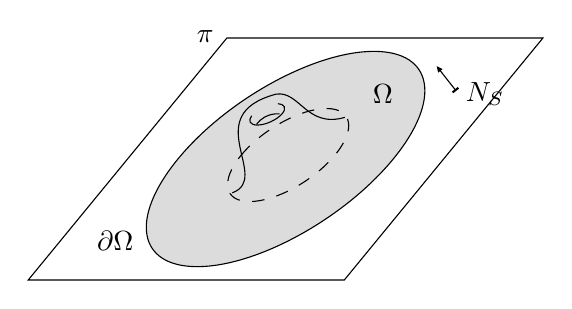
\begin{tikzpicture}[x=0.3pt,y=0.3pt,yscale=-1,xscale=1]
%uncomment if require: \path (0,361); %set diagram left start at 0, and has height of 361

%Shape: Circle [id:dp9482348629253332] 
\draw  [fill={rgb, 255:red, 155; green, 155; blue, 155 }  ,fill opacity=0.35 ] (200.38,172.92) .. controls (259.16,101.31) and (364.86,43.26) .. (436.47,43.26) .. controls (508.08,43.26) and (518.48,101.31) .. (459.7,172.92) .. controls (400.92,244.53) and (295.22,302.58) .. (223.61,302.58) .. controls (152,302.58) and (141.6,244.53) .. (200.38,172.92) -- cycle ;
%Shape: Rectangle [id:dp2870763717907634] 
\draw   (259.33,27.17) -- (640.02,27.17) -- (400.75,318.67) -- (20.06,318.67) -- cycle ;
%Shape: Ellipse [id:dp2652508582533277] 
\draw  [dash pattern={on 4.5pt off 4.5pt}] (276.72,168.15) .. controls (302.29,137.21) and (348.27,112.13) .. (379.41,112.13) .. controls (410.56,112.13) and (415.09,137.21) .. (389.52,168.15) .. controls (363.95,199.09) and (317.97,224.17) .. (286.83,224.17) .. controls (255.68,224.17) and (251.15,199.09) .. (276.72,168.15) -- cycle ;
%Curve Lines [id:da6223866126114177] 
\draw    (265.85,213.61) .. controls (314.03,196.1) and (224.08,120.17) .. (318.44,94.83) ;
%Curve Lines [id:da9304215465781236] 
\draw    (318.44,94.83) .. controls (347.08,90.17) and (355.08,136.17) .. (401.43,122.78) ;
%Shape: Arc [id:dp1565208649499492] 
\draw  [draw opacity=0] (320.77,106.3) .. controls (324.51,106.45) and (327.31,107.59) .. (328.42,109.71) .. controls (330.94,114.55) and (323.81,122.69) .. (312.49,127.9) .. controls (301.17,133.12) and (289.95,133.42) .. (287.42,128.59) .. controls (286.31,126.46) and (287.07,123.69) .. (289.23,120.81) -- (307.92,119.15) -- cycle ; \draw   (320.77,106.3) .. controls (324.51,106.45) and (327.31,107.59) .. (328.42,109.71) .. controls (330.94,114.55) and (323.81,122.69) .. (312.49,127.9) .. controls (301.17,133.12) and (289.95,133.42) .. (287.42,128.59) .. controls (286.31,126.46) and (287.07,123.69) .. (289.23,120.81) ;  
%Shape: Arc [id:dp6518966060475648] 
\draw  [draw opacity=0] (295.3,130.79) .. controls (297.67,127.56) and (300.8,124.73) .. (304.6,122.57) .. controls (310.34,119.31) and (316.76,118.03) .. (322.96,118.52) -- (320.41,147.08) -- cycle ; \draw   (295.3,130.79) .. controls (297.67,127.56) and (300.8,124.73) .. (304.6,122.57) .. controls (310.34,119.31) and (316.76,118.03) .. (322.96,118.52) ;  
%Straight Lines [id:da6781144891006192] 
\draw    (534.7,89.92) -- (513.94,63.53) ;
\draw [shift={(512.08,61.17)}, rotate = 51.8] [fill={rgb, 255:red, 0; green, 0; blue, 0 }  ][line width=0.08]  [draw opacity=0] (7.14,-3.43) -- (0,0) -- (7.14,3.43) -- cycle    ;
\draw [shift={(534.7,89.92)}, rotate = 51.8] [color={rgb, 255:red, 0; green, 0; blue, 0 }  ][line width=0.75]    (0,4.47) -- (0,-4.47)   ;

% Text Node
\draw (432,80.4) node [anchor=north west][inner sep=0.75pt]    {$\Omega $};
% Text Node
\draw (100,257.4) node [anchor=north west][inner sep=0.75pt]    {$\partial \Omega $};
% Text Node
\draw (544,77.4) node [anchor=north west][inner sep=0.75pt]    {$N_{S}$};
% Text Node
\draw (220,15.4) node [anchor=north west][inner sep=0.75pt]    {$\pi $};


\end{tikzpicture}

    \end{center}
    \caption{Superficie regular $\Omega$ que es subconjunto de $S$}
    \label{fig:problemafinal1}
\end{figure}
\\ Notemos que al ser $S$ una superficie cerrada, la única frontera del subconjunto $\Omega$ será el círculo que la delimita, y escogiendo la orientación adecuada tendremos que $k_g\equiv \frac{1}{R}$ en $\partial\Omega$ y de esto, por el teorema de Gauss Bonnet
\begin{align}
    \int_{\partial\Omega} k_g+\int\int_\Omega K&=2\pi\chi(\Omega)\notag\\
    \int\int_\Omega K&=2\pi\chi(\Omega)-\int_{0}^{2\pi R} \dfrac{1}{R}ds\notag \\
    &=2\pi\left(\chi(\Omega)-1)\right)\label{eq: GB1} 
\end{align}
 como se supone $K\geq 0$, la integral será no negativa también y $\chi(\Omega)\geq 1$. Mostraremos que efectivamente $\chi(\Omega)=1$. Notemos que podemos tomar esta superficie $\Omega$ y volverla compacta de la siguiente forma, si tomamos los segmentos que unen la frontera de $\Omega$ y el circulo de radio $R$ contenido en $\pi$ a lo largo del eje $y$, unimos los bordes exteriores con una curva regular contenida en el plano $yz$ y luego giramos esa curva alrededor del eje $z$ tendremos una superficie regular compacta como en Figura \ref{fig:problemafinal2}, a esta la llamaremos $\Omega'$. \\

 \begin{figure}[h]
    \begin{center}
        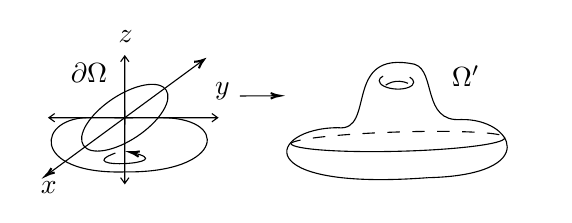
\begin{tikzpicture}[x=0.3pt,y=0.3pt,yscale=-1,xscale=1]
%uncomment if require: \path (0,251); %set diagram left start at 0, and has height of 251

%Shape: Axis 2D [id:dp5910562948647893] 
\draw  (133,118.16) -- (257.32,118.16)(145.43,43.74) -- (145.43,126.43) (250.32,113.16) -- (257.32,118.16) -- (250.32,123.16) (140.43,50.74) -- (145.43,43.74) -- (150.43,50.74)  ;
%Shape: Axis 2D [id:dp23965733482851959] 
\draw  (155.58,118.16) -- (54.02,118.16)(145.42,197.37) -- (145.42,109.36) (61.02,123.16) -- (54.02,118.16) -- (61.02,113.16) (150.42,190.37) -- (145.42,197.37) -- (140.42,190.37)  ;
%Straight Lines [id:da81728975332874] 
\draw    (239.01,49.46) -- (51.84,186.86) ;
\draw [shift={(50.23,188.05)}, rotate = 323.72] [color={rgb, 255:red, 0; green, 0; blue, 0 }  ][line width=0.75]    (10.93,-3.29) .. controls (6.95,-1.4) and (3.31,-0.3) .. (0,0) .. controls (3.31,0.3) and (6.95,1.4) .. (10.93,3.29)   ;
\draw [shift={(240.63,48.28)}, rotate = 143.72] [color={rgb, 255:red, 0; green, 0; blue, 0 }  ][line width=0.75]    (10.93,-4.9) .. controls (6.95,-2.3) and (3.31,-0.67) .. (0,0) .. controls (3.31,0.67) and (6.95,2.3) .. (10.93,4.9)   ;
%Shape: Ellipse [id:dp3915301339342794] 
\draw   (105.22,118.16) .. controls (123.44,95.96) and (156.22,77.96) .. (178.42,77.96) .. controls (200.62,77.96) and (203.85,95.96) .. (185.62,118.16) .. controls (167.4,140.37) and (134.62,158.37) .. (112.42,158.37) .. controls (90.22,158.37) and (86.99,140.37) .. (105.22,118.16) -- cycle ;
%Curve Lines [id:da39019357925175635] 
\draw    (185.62,118.16) .. controls (273.37,116.24) and (266.14,184.89) .. (146.18,183.44) ;
%Curve Lines [id:da5809295372195042] 
\draw    (105.22,118.16) .. controls (39.55,115.51) and (29.12,187.05) .. (146.18,183.44) ;
%Curve Lines [id:da16099183522027016] 
\draw    (134.08,160.73) .. controls (77.65,181.52) and (216.26,173.89) .. (154.03,160.15) ;
\draw [shift={(152.08,159.73)}, rotate = 11.8] [color={rgb, 255:red, 0; green, 0; blue, 0 }  ][line width=0.75]    (10.93,-3.29) .. controls (6.95,-1.4) and (3.31,-0.3) .. (0,0) .. controls (3.31,0.3) and (6.95,1.4) .. (10.93,3.29)   ;
%Straight Lines [id:da9586405539021363] 
\draw    (284,92) -- (330.08,91.74) ;
\draw [shift={(332.08,91.73)}, rotate = 179.68] [color={rgb, 255:red, 0; green, 0; blue, 0 }  ][line width=0.75]    (10.93,-3.29) .. controls (6.95,-1.4) and (3.31,-0.3) .. (0,0) .. controls (3.31,0.3) and (6.95,1.4) .. (10.93,3.29)   ;
%Curve Lines [id:da1264527021818962] 
\draw    (401.99,130.18) .. controls (448.87,135.97) and (406.68,35.11) .. (494.78,53.86) ;
%Curve Lines [id:da04762517205971295] 
\draw    (494.78,53.86) .. controls (520.24,62.06) and (503.58,123.67) .. (550.24,120.38) ;
%Shape: Arc [id:dp949949606907339] 
\draw  [draw opacity=0] (488.61,69.29) .. controls (491.59,70.99) and (493.38,73.09) .. (493.41,75.31) .. controls (493.46,80.38) and (484.2,84.13) .. (472.73,83.68) .. controls (461.25,83.23) and (451.91,78.76) .. (451.85,73.68) .. controls (451.83,71.47) and (453.59,69.5) .. (456.53,68.03) -- (472.63,74.5) -- cycle ; \draw   (488.61,69.29) .. controls (491.59,70.99) and (493.38,73.09) .. (493.41,75.31) .. controls (493.46,80.38) and (484.2,84.13) .. (472.73,83.68) .. controls (461.25,83.23) and (451.91,78.76) .. (451.85,73.68) .. controls (451.83,71.47) and (453.59,69.5) .. (456.53,68.03) ;  
%Curve Lines [id:da36695516537401063] 
\draw    (550.24,120.38) .. controls (612.93,118.63) and (649.87,187.39) .. (509.96,190.43) ;
%Curve Lines [id:da9264934039292583] 
\draw    (401.99,130.18) .. controls (317.26,130.75) and (292.81,206.76) .. (509.96,190.43) ;
%Shape: Arc [id:dp15792453496863068] 
\draw  [draw opacity=0] (459.69,78.94) .. controls (464.28,75.76) and (470,74.01) .. (476.22,74.3) .. controls (479.88,74.47) and (483.39,75.33) .. (486.6,76.75) -- (476.47,101.42) -- cycle ; \draw   (459.69,78.94) .. controls (464.28,75.76) and (470,74.01) .. (476.22,74.3) .. controls (479.88,74.47) and (483.39,75.33) .. (486.6,76.75) ;  
%Shape: Arc [id:dp9534024368305363] 
\draw  [draw opacity=0] (602.56,141.4) .. controls (602.89,141.77) and (603.05,142.15) .. (603.04,142.53) .. controls (602.93,149.68) and (545.14,156.89) .. (473.96,158.64) .. controls (405.11,160.34) and (348.95,156.3) .. (345.46,149.57) -- (474.16,145.71) -- cycle ; \draw   (602.56,141.4) .. controls (602.89,141.77) and (603.05,142.15) .. (603.04,142.53) .. controls (602.93,149.68) and (545.14,156.89) .. (473.96,158.64) .. controls (405.11,160.34) and (348.95,156.3) .. (345.46,149.57) ;  
%Shape: Arc [id:dp6383081999291902] 
\draw  [draw opacity=0][dash pattern={on 4.5pt off 4.5pt}] (596.49,138.68) .. controls (579.94,135.03) and (531.41,133.56) .. (474.07,135.38) .. controls (405.92,137.54) and (350.09,143.58) .. (345.57,149.12) -- (473.91,145.73) -- cycle ; \draw  [dash pattern={on 4.5pt off 4.5pt}] (596.49,138.68) .. controls (579.94,135.03) and (531.41,133.56) .. (474.07,135.38) .. controls (405.92,137.54) and (350.09,143.58) .. (345.57,149.12) ;  

% Text Node
\draw (41.29,191.64) node [anchor=north west][inner sep=0.75pt]    {$x$};
% Text Node
\draw (251.02,72.24) node [anchor=north west][inner sep=0.75pt]    {$y$};
% Text Node
\draw (134.71,10.39) node [anchor=north west][inner sep=0.75pt]    {$z$};
% Text Node
\draw (77.27,49.93) node [anchor=north west][inner sep=0.75pt]    {$\partial \Omega $};
% Text Node
\draw (536.27,51.93) node [anchor=north west][inner sep=0.75pt]    {$\Omega '$};


\end{tikzpicture}
    \end{center}
    \caption{Nueva superficie $\Omega'$ generada con $\Omega$.}
    \label{fig:problemafinal2}
\end{figure}
 Ahora, para calcular la característica de Euler de $\Omega'$ (ver Figura \ref{fig:problemafinal3}) tomaremos una triangulación de $\Omega$, si consideramos todos los vértices en $\partial\Omega$, con eso podremos triangular el resto de la superficie, uniendo cada uno de estos vértices con un punto en $\Omega'/\overline{\Omega}$ mediante partes de meridianos de la parte inferior de $\Omega'$, con eso podremos obtener la relación $\chi(\Omega')=\chi(\Omega)+1$, pues por cada artista agregada hay una única cara agregada, y solamente un vértice extra en total.
  \begin{figure}[h]
    \begin{center}
        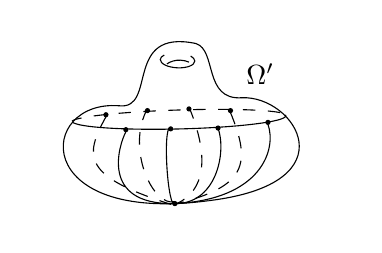
\begin{tikzpicture}[x=0.3pt,y=0.3pt,yscale=-1,xscale=1]
%uncomment if require: \path (0,300); %set diagram left start at 0, and has height of 300

%Curve Lines [id:da6897269523977254] 
\draw    (248.99,106.74) .. controls (295.87,112.42) and (253.68,13.37) .. (341.78,31.78) ;
%Curve Lines [id:da39198775641462347] 
\draw    (341.78,31.78) .. controls (367.24,39.84) and (350.58,100.34) .. (397.24,97.11) ;
%Shape: Arc [id:dp8537644214677098] 
\draw  [draw opacity=0] (335.49,46.87) .. controls (338.54,48.55) and (340.38,50.64) .. (340.41,52.85) .. controls (340.46,57.83) and (331.2,61.51) .. (319.73,61.07) .. controls (308.25,60.63) and (298.91,56.23) .. (298.85,51.25) .. controls (298.83,49.05) and (300.63,47.1) .. (303.64,45.65) -- (319.63,52.05) -- cycle ; \draw   (335.49,46.87) .. controls (338.54,48.55) and (340.38,50.64) .. (340.41,52.85) .. controls (340.46,57.83) and (331.2,61.51) .. (319.73,61.07) .. controls (308.25,60.63) and (298.91,56.23) .. (298.85,51.25) .. controls (298.83,49.05) and (300.63,47.1) .. (303.64,45.65) ;  
%Curve Lines [id:da25906896433123405] 
\draw    (397.24,97.13) .. controls (459.93,94.04) and (531.08,200.17) .. (356.96,221.1) ;
%Curve Lines [id:da7757860861524872] 
\draw    (248.99,106.74) .. controls (151.08,99.42) and (139.81,250) .. (356.96,221.1) ;
%Shape: Arc [id:dp9468374804856692] 
\draw  [draw opacity=0] (306.88,56.29) .. controls (311.44,53.24) and (317.08,51.57) .. (323.22,51.85) .. controls (326.82,52.02) and (330.27,52.84) .. (333.44,54.19) -- (323.47,78.49) -- cycle ; \draw   (306.88,56.29) .. controls (311.44,53.24) and (317.08,51.57) .. (323.22,51.85) .. controls (326.82,52.02) and (330.27,52.84) .. (333.44,54.19) ;  
%Shape: Arc [id:dp34327761973516724] 
\draw  [draw opacity=0] (449.55,117.75) .. controls (449.88,118.12) and (450.05,118.5) .. (450.04,118.88) .. controls (449.93,125.91) and (392.14,132.99) .. (320.96,134.7) .. controls (253.76,136.32) and (198.65,132.58) .. (192.8,126.24) -- (321.16,121.99) -- cycle ; \draw   (449.55,117.75) .. controls (449.88,118.12) and (450.05,118.5) .. (450.04,118.88) .. controls (449.93,125.91) and (392.14,132.99) .. (320.96,134.7) .. controls (253.76,136.32) and (198.65,132.58) .. (192.8,126.24) ;  
%Shape: Arc [id:dp1020919976874346] 
\draw  [draw opacity=0][dash pattern={on 4.5pt off 4.5pt}] (443.27,115.03) .. controls (426.53,111.49) and (378.17,110.07) .. (321.07,111.85) .. controls (252.98,113.98) and (197.18,119.9) .. (192.58,125.33) -- (320.91,122.01) -- cycle ; \draw  [dash pattern={on 4.5pt off 4.5pt}] (443.27,115.03) .. controls (426.53,111.49) and (378.17,110.07) .. (321.07,111.85) .. controls (252.98,113.98) and (197.18,119.9) .. (192.58,125.33) ;  
%Shape: Circle [id:dp24432163602662604] 
\draw  [fill={rgb, 255:red, 0; green, 0; blue, 0 }  ,fill opacity=1 ] (231,117.58) .. controls (231,116.25) and (232.08,115.17) .. (233.42,115.17) .. controls (234.75,115.17) and (235.83,116.25) .. (235.83,117.58) .. controls (235.83,118.92) and (234.75,120) .. (233.42,120) .. controls (232.08,120) and (231,118.92) .. (231,117.58) -- cycle ;
%Shape: Circle [id:dp12436585137166278] 
\draw  [fill={rgb, 255:red, 0; green, 0; blue, 0 }  ,fill opacity=1 ] (281,112.58) .. controls (281,111.25) and (282.08,110.17) .. (283.42,110.17) .. controls (284.75,110.17) and (285.83,111.25) .. (285.83,112.58) .. controls (285.83,113.92) and (284.75,115) .. (283.42,115) .. controls (282.08,115) and (281,113.92) .. (281,112.58) -- cycle ;
%Shape: Circle [id:dp6009294356821708] 
\draw  [fill={rgb, 255:red, 0; green, 0; blue, 0 }  ,fill opacity=1 ] (331,110.58) .. controls (331,109.25) and (332.08,108.17) .. (333.42,108.17) .. controls (334.75,108.17) and (335.83,109.25) .. (335.83,110.58) .. controls (335.83,111.92) and (334.75,113) .. (333.42,113) .. controls (332.08,113) and (331,111.92) .. (331,110.58) -- cycle ;
%Shape: Circle [id:dp1535261918981996] 
\draw  [fill={rgb, 255:red, 0; green, 0; blue, 0 }  ,fill opacity=1 ] (381,112.58) .. controls (381,111.25) and (382.08,110.17) .. (383.42,110.17) .. controls (384.75,110.17) and (385.83,111.25) .. (385.83,112.58) .. controls (385.83,113.92) and (384.75,115) .. (383.42,115) .. controls (382.08,115) and (381,113.92) .. (381,112.58) -- cycle ;
%Shape: Circle [id:dp35036097958490786] 
\draw  [fill={rgb, 255:red, 0; green, 0; blue, 0 }  ,fill opacity=1 ] (255,135.58) .. controls (255,134.25) and (256.08,133.17) .. (257.42,133.17) .. controls (258.75,133.17) and (259.83,134.25) .. (259.83,135.58) .. controls (259.83,136.92) and (258.75,138) .. (257.42,138) .. controls (256.08,138) and (255,136.92) .. (255,135.58) -- cycle ;
%Shape: Circle [id:dp15290975131352424] 
\draw  [fill={rgb, 255:red, 0; green, 0; blue, 0 }  ,fill opacity=1 ] (309,134.58) .. controls (309,133.25) and (310.08,132.17) .. (311.42,132.17) .. controls (312.75,132.17) and (313.83,133.25) .. (313.83,134.58) .. controls (313.83,135.92) and (312.75,137) .. (311.42,137) .. controls (310.08,137) and (309,135.92) .. (309,134.58) -- cycle ;
%Shape: Circle [id:dp9544372227346376] 
\draw  [fill={rgb, 255:red, 0; green, 0; blue, 0 }  ,fill opacity=1 ] (366,133.58) .. controls (366,132.25) and (367.08,131.17) .. (368.42,131.17) .. controls (369.75,131.17) and (370.83,132.25) .. (370.83,133.58) .. controls (370.83,134.92) and (369.75,136) .. (368.42,136) .. controls (367.08,136) and (366,134.92) .. (366,133.58) -- cycle ;
%Shape: Circle [id:dp7508779290729328] 
\draw  [fill={rgb, 255:red, 0; green, 0; blue, 0 }  ,fill opacity=1 ] (426.13,126.75) .. controls (426.13,125.42) and (427.21,124.34) .. (428.55,124.34) .. controls (429.88,124.34) and (430.96,125.42) .. (430.96,126.75) .. controls (430.96,128.09) and (429.88,129.17) .. (428.55,129.17) .. controls (427.21,129.17) and (426.13,128.09) .. (426.13,126.75) -- cycle ;
%Shape: Circle [id:dp091865733865643] 
\draw  [fill={rgb, 255:red, 0; green, 0; blue, 0 }  ,fill opacity=1 ] (314,224.58) .. controls (314,223.25) and (315.08,222.17) .. (316.42,222.17) .. controls (317.75,222.17) and (318.83,223.25) .. (318.83,224.58) .. controls (318.83,225.92) and (317.75,227) .. (316.42,227) .. controls (315.08,227) and (314,225.92) .. (314,224.58) -- cycle ;
%Curve Lines [id:da7394429921377821] 
\draw    (257.42,138) .. controls (249.08,154.17) and (226.08,225.17) .. (314,224.58) ;
%Curve Lines [id:da41964067239816827] 
\draw    (309,134.58) .. controls (302.08,148.17) and (309.08,242.17) .. (318.83,224.58) ;
%Curve Lines [id:da6417292398311423] 
\draw    (368.42,133.58) .. controls (379.08,163.17) and (366.08,227.17) .. (314,224.58) ;
%Curve Lines [id:da9016112010439528] 
\draw    (428.55,129.17) .. controls (439.21,158.75) and (421.08,219.75) .. (316.42,224.58) ;
%Curve Lines [id:da2245958643931525] 
\draw  [dash pattern={on 4.5pt off 4.5pt}]  (233.42,120) .. controls (207.08,168.17) and (204.08,192.17) .. (316.42,227) ;
%Curve Lines [id:da8925283948537885] 
\draw  [dash pattern={on 4.5pt off 4.5pt}]  (283.42,110.17) .. controls (257.08,158.34) and (290.08,229.17) .. (316.42,222.17) ;
%Curve Lines [id:da4132142241147987] 
\draw  [dash pattern={on 4.5pt off 4.5pt}]  (333.42,108.17) .. controls (359.08,170.17) and (352.08,209.17) .. (318.83,224.58) ;
%Curve Lines [id:da8080243759401962] 
\draw  [dash pattern={on 4.5pt off 4.5pt}]  (383.42,115) .. controls (409.08,177) and (402.08,204.17) .. (318.83,224.58) ;

% Text Node
\draw (399.27,52.75) node [anchor=north west][inner sep=0.75pt]    {$\Omega '$};


\end{tikzpicture}

    \end{center}
     \caption{Nueva triangulación para calcular $\chi(\Omega')$.}
     \label{fig:problemafinal3}
 \end{figure}
 \\ De la primera parte tendremos
\begin{align*}
    \chi(\Omega')=\chi(\Omega)+1\geq 2
\end{align*}
y la característica de Euler de una superficie compacta conexa solo puede ser $2,0,-2,-4,...$ se tendrá que $\chi(\Omega')=2$ y por tanto $\chi(\Omega)=1$, de lo que se puede concluir que $\Omega$ es homeomorfo a un disco, es decir, es una región simple regular, pero además por \ref{eq: GB1} se tiene
\begin{align*}
    \int\int_\Omega K=0
\end{align*}
y como $K\geq 0$ se obtiene que $K\equiv 0$. Ahora mostraremos que efectivamente dentro de $B(R)$ es un plano. Ahora consideremos el punto dentro de $\overline{\Omega}$ más alejado del plano $xy$, este sabemos que existe pues $\overline{\Omega}$ es un conjunto cerrado, como está acotado, es un compacto, y si definimos la función distancia del plano $xy$ de la superficie, esta será continua y como está definida en un compacto sabemos que alcanza su máximo. Supongamos que ese máximo ocurre en $P=(x,y,z_0)$, si $z_0\neq 0$, sin pérdida de generalidad supondremos $z_0>0$, pues si $z_0<0$ solamente cambiamos el eje $+z$ por el $-z$. Si tomamos $\Omega'$ nuevamente (que ahora sabemos que tiene la topología de una esfera) y una esfera $S_R$ centrada en un punto que variable del eje $z$ con un radio $R$ fijo lo suficientemente grande para que toque $P$ pero no toque $\partial \Omega$ y $\Omega'$ esté contenida en $S_R$ notemos que esto solamente se puede hacer de manera que $\Omega'$ esté contenido en la esfera cuando $z_0>0$, pues el radio de la esfera variará inversamente proporcional a $z_0$, como podemos ver en la Figura \ref{fig:problemafinal4}
\begin{figure}[h]
    \begin{center}
        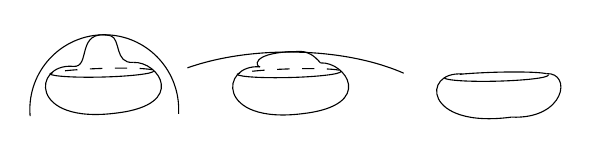
\begin{tikzpicture}[x=0.35pt,y=0.35pt,yscale=-1,xscale=1]
%uncomment if require: \path (0,227); %set diagram left start at 0, and has height of 227

%Curve Lines [id:da1034317952128736] 
\draw    (103.21,88.04) .. controls (122.96,90.43) and (105.19,48.7) .. (142.3,56.46) ;
%Curve Lines [id:da33258074413270955] 
\draw    (142.3,56.46) .. controls (153.03,59.85) and (146.01,85.34) .. (165.67,83.98) ;
%Curve Lines [id:da8866701934647774] 
\draw    (165.67,83.99) .. controls (192.08,82.69) and (222.05,127.4) .. (148.7,136.22) ;
%Curve Lines [id:da024480663990893436] 
\draw    (103.21,88.04) .. controls (61.96,84.96) and (57.21,148.39) .. (148.7,136.22) ;
%Shape: Arc [id:dp9849479313078455] 
\draw  [draw opacity=0] (186.51,92.35) .. controls (186.67,92.51) and (186.75,92.66) .. (186.74,92.82) .. controls (186.7,95.59) and (162.62,98.4) .. (132.95,99.12) .. controls (105.05,99.79) and (82.15,98.36) .. (79.57,95.89) -- (133.03,94.12) -- cycle ; \draw   (186.51,92.35) .. controls (186.67,92.51) and (186.75,92.66) .. (186.74,92.82) .. controls (186.7,95.59) and (162.62,98.4) .. (132.95,99.12) .. controls (105.05,99.79) and (82.15,98.36) .. (79.57,95.89) ;  
%Shape: Arc [id:dp05324828240555979] 
\draw  [draw opacity=0][dash pattern={on 4.5pt off 4.5pt}] (185.06,91.53) .. controls (178,90.04) and (157.63,89.44) .. (133.58,90.19) .. controls (104.89,91.09) and (81.38,93.58) .. (79.44,95.87) -- (133.51,94.47) -- cycle ; \draw  [dash pattern={on 4.5pt off 4.5pt}] (185.06,91.53) .. controls (178,90.04) and (157.63,89.44) .. (133.58,90.19) .. controls (104.89,91.09) and (81.38,93.58) .. (79.44,95.87) ;  
%Curve Lines [id:da9023608124375635] 
\draw    (296.5,88.53) .. controls (292.39,88.67) and (286.38,75.14) .. (327.71,72.88) ;
%Curve Lines [id:da4727999724530163] 
\draw    (327.71,72.88) .. controls (336.73,73.63) and (345,68.37) .. (358.95,84.48) ;
%Curve Lines [id:da2922563351921048] 
\draw    (358.95,84.49) .. controls (385.36,83.18) and (415.34,127.9) .. (341.98,136.71) ;
%Curve Lines [id:da9795001489559958] 
\draw    (296.5,88.53) .. controls (255.25,85.45) and (250.5,148.89) .. (341.98,136.71) ;
%Shape: Arc [id:dp7918098543989271] 
\draw  [draw opacity=0] (379.8,92.85) .. controls (379.95,93) and (380.03,93.16) .. (380.03,93.32) .. controls (379.99,96.08) and (355.9,98.9) .. (326.24,99.61) .. controls (298.34,100.29) and (275.43,98.86) .. (272.85,96.39) -- (326.32,94.61) -- cycle ; \draw   (379.8,92.85) .. controls (379.95,93) and (380.03,93.16) .. (380.03,93.32) .. controls (379.99,96.08) and (355.9,98.9) .. (326.24,99.61) .. controls (298.34,100.29) and (275.43,98.86) .. (272.85,96.39) ;  
%Shape: Arc [id:dp5166424159947098] 
\draw  [draw opacity=0][dash pattern={on 4.5pt off 4.5pt}] (378.35,92.03) .. controls (371.29,90.54) and (350.92,89.94) .. (326.86,90.69) .. controls (298.18,91.58) and (274.67,94.08) .. (272.73,96.37) -- (326.8,94.97) -- cycle ; \draw  [dash pattern={on 4.5pt off 4.5pt}] (378.35,92.03) .. controls (371.29,90.54) and (350.92,89.94) .. (326.86,90.69) .. controls (298.18,91.58) and (274.67,94.08) .. (272.73,96.37) ;  
%Curve Lines [id:da24947666426214044] 
\draw    (592.2,95.56) .. controls (618.61,94.25) and (612.08,142.97) .. (556.03,140.48) ;
%Curve Lines [id:da82695706364757] 
\draw    (505.08,95.97) .. controls (463.83,92.89) and (464.54,152.65) .. (556.03,140.48) ;
%Shape: Arc [id:dp7136846011757716] 
\draw  [draw opacity=0] (593.84,96.62) .. controls (594,96.77) and (594.08,96.92) .. (594.07,97.08) .. controls (594.03,99.85) and (569.95,102.66) .. (540.29,103.38) .. controls (512.38,104.05) and (489.48,102.62) .. (486.9,100.15) -- (540.37,98.38) -- cycle ; \draw   (593.84,96.62) .. controls (594,96.77) and (594.08,96.92) .. (594.07,97.08) .. controls (594.03,99.85) and (569.95,102.66) .. (540.29,103.38) .. controls (512.38,104.05) and (489.48,102.62) .. (486.9,100.15) ;  
%Shape: Arc [id:dp8673306382519155] 
\draw  [draw opacity=0] (592.2,95.56) .. controls (584.73,94.01) and (563.34,93.4) .. (538.09,94.19) .. controls (524.89,94.6) and (512.73,95.33) .. (503.06,96.22) -- (538.02,98.65) -- cycle ; \draw   (592.2,95.56) .. controls (584.73,94.01) and (563.34,93.4) .. (538.09,94.19) .. controls (524.89,94.6) and (512.73,95.33) .. (503.06,96.22) ;  
%Shape: Arc [id:dp3654479329689415] 
\draw  [draw opacity=0] (59.17,139.37) .. controls (58.98,137.13) and (58.88,134.87) .. (58.88,132.58) .. controls (58.89,89.96) and (93.3,55.43) .. (135.74,55.44) .. controls (178.17,55.45) and (212.56,90.01) .. (212.54,132.63) .. controls (212.54,134.13) and (212.5,135.63) .. (212.41,137.11) -- (135.71,132.6) -- cycle ; \draw   (59.17,139.37) .. controls (58.98,137.13) and (58.88,134.87) .. (58.88,132.58) .. controls (58.89,89.96) and (93.3,55.43) .. (135.74,55.44) .. controls (178.17,55.45) and (212.56,90.01) .. (212.54,132.63) .. controls (212.54,134.13) and (212.5,135.63) .. (212.41,137.11) ;  
%Shape: Arc [id:dp6974572340273233] 
\draw  [draw opacity=0] (221.54,89.63) .. controls (250.42,79.37) and (286.81,73.27) .. (326.35,73.28) .. controls (372.45,73.3) and (414.27,81.63) .. (444.9,95.15) -- (326.32,150.44) -- cycle ; \draw   (221.54,89.63) .. controls (250.42,79.37) and (286.81,73.27) .. (326.35,73.28) .. controls (372.45,73.3) and (414.27,81.63) .. (444.9,95.15) ;  




\end{tikzpicture}
    \end{center}
    \caption{Construcción $S_R$, en la tercera figura la esfera debería tener un radio infinito.}
    \label{fig:problemafinal4}
\end{figure}
\\ 

Ahora si vamos variando (bajando) el centro de la esfera a lo largo del eje $z$ debe existir al menos un primer punto de contacto, porque $\Omega'$ es un conjunto compacto, y por la construcción que se hizo para la esfera debe ser necesariamente un punto de $\Omega$ como en las primeras dos superficies de la Figura \ref{fig:problemafinal4}. Al ser un primer punto de contacto, debe ocurrir que los planos tangentes coinciden y podremos comparar las superficies como en la Figura \ref{fig:problemafinal5}.
\begin{figure}[h]
    \begin{center}
      

\begin{tikzpicture}[x=0.7pt,y=0.7pt,yscale=-1,xscale=1]
%uncomment if require: \path (0,300); %set diagram left start at 0, and has height of 300

%Curve Lines [id:da0471946465083628] 
\draw    (281.22,95.05) .. controls (272.67,113.02) and (316.03,108.6) .. (296.87,141.32) ;
%Curve Lines [id:da4358913791921397] 
\draw    (296.87,141.32) .. controls (290.24,150.41) and (263.69,151.28) .. (258.73,170.35) ;
%Shape: Arc [id:dp5550271873705848] 
\draw  [draw opacity=0] (250.72,184.57) .. controls (250.52,184.67) and (250.35,184.69) .. (250.2,184.64) .. controls (247.59,183.72) and (252.58,159.99) .. (261.33,131.64) .. controls (270.09,103.29) and (279.3,81.05) .. (281.9,81.97) .. controls (283.05,82.38) and (282.72,87.27) .. (281.22,95.05) -- (266.05,133.3) -- cycle ; \draw   (250.72,184.57) .. controls (250.52,184.67) and (250.35,184.69) .. (250.2,184.64) .. controls (247.59,183.72) and (252.58,159.99) .. (261.33,131.64) .. controls (270.09,103.29) and (279.3,81.05) .. (281.9,81.97) .. controls (283.05,82.38) and (282.72,87.27) .. (281.22,95.05) ;  
%Shape: Arc [id:dp7329537141949276] 
\draw  [draw opacity=0] (250.72,184.57) .. controls (250.8,184.86) and (250.93,185.04) .. (251.09,185.09) .. controls (252.22,185.5) and (255.07,179.82) .. (258.73,170.35) -- (266.71,133.17) -- cycle ; \draw   (250.72,184.57) .. controls (250.8,184.86) and (250.93,185.04) .. (251.09,185.09) .. controls (252.22,185.5) and (255.07,179.82) .. (258.73,170.35) ;  
%Shape: Arc [id:dp7316628168241703] 
\draw  [draw opacity=0] (242.64,44.88) .. controls (244.82,45.41) and (247,46.04) .. (249.17,46.77) .. controls (289.57,60.33) and (311.37,103.94) .. (297.86,144.16) .. controls (284.35,184.39) and (240.65,206) .. (200.25,192.44) .. controls (198.83,191.96) and (197.43,191.45) .. (196.05,190.89) -- (224.71,119.6) -- cycle ; \draw   (242.64,44.88) .. controls (244.82,45.41) and (247,46.04) .. (249.17,46.77) .. controls (289.57,60.33) and (311.37,103.94) .. (297.86,144.16) .. controls (284.35,184.39) and (240.65,206) .. (200.25,192.44) .. controls (198.83,191.96) and (197.43,191.45) .. (196.05,190.89) ;  
%Shape: Circle [id:dp010845998360254683] 
\draw  [fill={rgb, 255:red, 0; green, 0; blue, 0 }  ,fill opacity=1 ] (221.42,122.65) .. controls (221.42,122.52) and (221.52,122.41) .. (221.66,122.41) .. controls (221.79,122.41) and (221.9,122.52) .. (221.9,122.65) .. controls (221.9,122.79) and (221.79,122.9) .. (221.66,122.9) .. controls (221.52,122.9) and (221.42,122.79) .. (221.42,122.65) -- cycle ;
%Straight Lines [id:da4106283479028623] 
\draw    (221.42,122.65) -- (268.27,60.8) ;
\draw [shift={(270.08,58.41)}, rotate = 127.14] [fill={rgb, 255:red, 0; green, 0; blue, 0 }  ][line width=0.08]  [draw opacity=0] (8.93,-4.29) -- (0,0) -- (8.93,4.29) -- cycle    ;
%Shape: Rectangle [id:dp7827143611696217] 
\draw  [fill={rgb, 255:red, 155; green, 155; blue, 155 }  ,fill opacity=0.32 ][dash pattern={on 0.84pt off 2.51pt}] (298.26,67.41) -- (339.31,67.41) -- (305.14,198.32) -- (264.09,198.32) -- cycle ;
%Shape: Circle [id:dp5023092116503174] 
\draw  [fill={rgb, 255:red, 0; green, 0; blue, 0 }  ,fill opacity=1 ] (300.17,131.07) .. controls (300.17,130.08) and (300.98,129.27) .. (301.97,129.27) .. controls (302.96,129.27) and (303.76,130.08) .. (303.76,131.07) .. controls (303.76,132.06) and (302.96,132.86) .. (301.97,132.86) .. controls (300.98,132.86) and (300.17,132.06) .. (300.17,131.07) -- cycle ;

% Text Node
\draw (223,74.4) node [anchor=north west][inner sep=0.75pt]    {$R$};
% Text Node
\draw (302.17,134.47) node [anchor=north west][inner sep=0.75pt]    {$Q$};
% Text Node
\draw (376,104.4) node [anchor=north west][inner sep=0.75pt]    {$K( Q) \geq \ \dfrac{1}{R^{2}}$};


\end{tikzpicture}
    \end{center}
    \caption{Comparación de dos superficies}
    \label{fig:problemafinal5}
\end{figure}
\\

Obteniendo así que en ese punto de contacto $K(Q)\geq \frac{1}{R^2}>0$, pero $K\equiv 0$, así que esto es una contradicción que viene de suponer $z_0\neq 0$. Así que $z_0$ debe ser nulo, así tenderemos que como la distancia máxima entre el plano $z=0$ y $S$ es 0 y por tanto dentro de $B(R)$ la superficie también es plana. \\

\textbf{Nota:} es posible dar una solución de este problema usando el primer teorema de la sección 5.8 de \cite{do2016differential}, sin embargo, esto requiere teoría más pesada y por ello se opta por la solución presentada en esta sección.
\section{Formas y Gauss Bonnet}
Sea $S\subset \mathbb{R}^3$ una superficie regular. Una \textbf{forma diferencial de grado }$k$ en un abierto en la topología del subespacio $V\subset S$, es una aplicación $\omega$ que asocia cada punto $p\in V$ una función $k-$lineal alternante 
\begin{align*}
\omega_p:T_pS\times\ldots\times T_pS\to \mathbb{R}
\end{align*}
y que, además de eso, es tal que para todos los campos suaves de vectores tangentes $W_1,\ldots,W_k:V\subset S\to \mathbb{R}^3$, la función $\omega(W_1,\ldots,W_k):p\in V\mapsto \omega_p(W_1(p),\ldots,W_k(p))\in \mathbb{R}$ es suave.\\

Por ejemplo, sea $W$ un campo vectorial suave de vectores tangentes a $S$. Entonces, la regla
\begin{align*}
    \omega_p(v)=\langle W(p),v\rangle \quad p\in V, v\in T_pS,
\end{align*}
define una forma diferencial $\omega$ de grado 1 en $S$, que llamamos \textit{forma diferencial dual} al campo $W$.\\
Una operación algebraica importante entre formas diferenciales es el \textit{producto exterior}. En esta sección calcularemos el diferencial exterior de dos formas $\omega$ y $\eta$ de grado 1, cuya definición es la forma diferencial $\omega\land \eta$ de grado 2, dada por
\begin{align*}
    (\omega\land\eta)_p(v,w)=\omega_p(v)\eta_p(w)-\omega_p(w)\eta_p(v)\\ p\in V,\quad v,w\in T_pS,
\end{align*}
Una operación importante que actúa sobre las formas diferenciales es el \textit{diferencial exterior}. Calcularemos aquí sólo el diferencial exterior de formas de grado 1, que es la forma diferencial
de grado 2 dado por
\begin{align*}
    d\omega(Z,W)=Z\omega(W)-W\omega(Z)-\omega([Z,W]).
\end{align*}
Aquí, $Z\omega(W)$ es una función que asocia a cada punto $p\in S$ la derivada de la función suave $\omega(X)$ en la dirección $Z(p)\in T_pS$. (También es una función suave, y se prueba directamente escribiendo esta función en coordenadas). Similarmente se define $W\omega(Z)$. Además, $[Z,W]$ es el \textit{corchete de Lie} entre dos campos, dado en coordenadas por la siguiente fórmula, si 
\begin{align*}
    Z&=\sum_ia^i\partial_iX,\\
    W&=\sum_ib^i\partial_iX,
\end{align*}
entonces
\begin{align*}
    [Z,W]=\sum_i\left(\sum_j(a^j\partial_jb^i-b^j\partial_ja^i)\right)\partial_iX.
\end{align*}
De esto tendremos
\begin{proposition}
    Sea $S$, una superficie regular en $\mathbb{R}^3$ y $Z,W$ dos campos suaves de vectores tangentes. Muestre que
    \begin{align*}
        \nabla_XY-\nabla_YX=[X,Y].
    \end{align*}
\end{proposition}
\textit{Demostración.}  Ejercicio
\hfill$\blacksquare$\\


Consideremos entonces un \textit{referencial ortonormal local} en $S$, esto es, campos suaves de vectores tangentes $e_1$ y $e_2$ definidos en una abierto $V$ de $S$ tales que, en cada punto $p\in V$, $\{e_1(p),e_2(p)\}$ es base ortonormal de $T_pS$. Asociados a este campo de vectores están las formas $\omega_1$ y $\omega_2$, respectivamente. Definimos también las formas diferenciales de grado 1 dadas por
\begin{align*}
    (\omega_{ij})_p(w)=\langle \nabla_w e_i, e_j\rangle \quad p\in V, w\in T_pS.
\end{align*}
Un ejercicio recomendado es el de mostrar que
\begin{align*}
    \omega_{ij}&=-\omega_{ji}\\
    d\omega_1&=\omega_{12}\land \omega_2\\
    d\omega_2&=\omega_{21}\land \omega_1.
\end{align*}
Y haciendo la siguiente cuenta
\begin{align*}
    d\omega_{12}(Z,W)&=Z\omega(W)-W\omega(Z)-\omega([Z,W])\\
    &=Z\langle \nabla_W e_1, e_2\rangle-W\langle \nabla_Z e_1, e_2\rangle\\
    &-\langle \nabla_{[Z,W]} e_1, e_2\rangle\\
    &=\langle\nabla_Z \nabla_W e_1, e_2\rangle+\langle\nabla_W e_1, \nabla_Z e_2\rangle\\
    &-\langle\nabla_W \nabla_Z e_1, e_2\rangle-\langle\nabla_Z e_1, \nabla_W e_2\rangle\\
    &-\langle \nabla_{[Z,W]} e_1, e_2\rangle\\
    &=\langle\nabla_W \nabla_Z e_1-\nabla_Z \nabla_W e_1\\
    &-\nabla_{[Z,W]} e_1, e_2\rangle,
\end{align*}
donde los términos $\langle\nabla_W e_1, \nabla_Z e_2\rangle$ se anulan porque $\nabla_We_i$ es ortogonal a $e_i$ para $i=1,2$ y por tanto $\nabla_We_i$ es paralelo a $e_j$ donde $i\neq j$ en $\{1,2\}$.
\begin{proposition}
    \begin{align*}
        \langle\nabla_W \nabla_Z e_1-\nabla_Z \nabla_W e_1-\nabla_{[Z,W]} e_1, e_2\rangle
        \\
        =K(\langle e_1,W\rangle\langle e_2,Z\rangle-\langle e_1,Z\rangle\langle e_2,W\rangle),
    \end{align*}
    donde $K$ es la curvatura Gaussiana de $S$.
\end{proposition}
\textit{Demostración.} Ejercicio\hfill $\blacksquare$\\

En general pueden no existir referenciales ortonormales globalmente definidos en superficies regulares compactas con borde (o sin borde) de $\mathbb{R}^3$. Siempre es posible, a pesar de ello, encontrar un referencial ortonormal adaptado a $\partial S$, en el sentido de que $a)$ $e_1$ es tangente a $\partial S$; y $b)$ $e_1$ está definido en $S\textbackslash P$, donde $P$ es un conjunto finito de puntos en $S \textbackslash \partial S$. Removiendo pequeñas bolas $B_\varepsilon^i$, al rededor de estos $k$ puntos, y suponiendo que $S$ es orientable de modo que $\omega_1\land \omega_2$ es un elemento de volumen donde está definido. El hecho de que $K$ sea continua en $S$ y el teorema de Stokes nos da la igualdad
\begin{align*}
    \int_S K dS&=\lim_{\varepsilon\to 0} \int_{S\textbackslash \cup B^i_\varepsilon} K \omega_1\land \omega_2\\
    &=-\int_{\partial S}\omega_{12}-\lim_{\varepsilon\to 0}\sum_{i=1}^k\int_{\partial B^i_\varepsilon}\omega_{12}
\end{align*}
Para comprender la integral de $\omega_{12}$ en la frontera, parametrizamos cada componente por longitud de arco y velocidad dada por $e_1$ (que fue elegida tangente a $\partial S$). Así, en cada componente tenemos una integral
\begin{align*}
    \int_0^{\ell_i}(\omega_{12})_{\alpha(s)}(\alpha'(s))ds\\
    =\int_0^{\ell_i}\left\langle\dfrac{D e_1}{ds}(s), e_2(\alpha(s))\right\rangle ds
\end{align*}
Calculamos por integración directa: Usando que $\alpha'(s)=e_1(\alpha(s))$, tenemos que $k_g(s)=\left\langle\dfrac{D e_1}{ds}(s), e_2\right\rangle$. (Una función angular constante con respecto a $e_1$ es una función constante $=0$). Luego
\begin{align*}
    \int_S K dS+\int_{\partial S} k_g= -\lim_{\varepsilon\to 0}\sum_{i=1}^k\int_{\partial B^i_\varepsilon}\omega_{12}
\end{align*}
Para comprender el límite, se recomienda consultar la discusión sobre el teorema del índice de Poincaré en los libros de Manfredo. Tener en cuenta que no depende de la elección de la referencia (El lado izquierdo no depende).\\

De esta manera obtenemos un resultado más general de Gauss Bonnet, usando formas diferenciales.
%%%%%%%%%%%%%%%%%%%%%%%%%%%%%%%%%%%%%%%%%%%
\section{Ejercicios}

%%%%%%%%%%%%%%%%%%%%%%%%%%%%%%%%%%%%%%%%%%%
\chapter*{Apéndice A: Orientación}
\addcontentsline{toc}{chapter}{Apéndice A: Orientación}
Sea $V$ un espacio vectorial real de dimensión finita $n\geq 1$. Sea $\mathcal{B}_0$ un conjunto de las \textit{bases ordenadas} de $V$, es decir el conjunto:
\begin{align*}
\mathcal{B}_0=\left\{(v_1,\ldots,v_n)\in V\times \ldots\times V|\right.\\
   \left. \text{span}\{v_1,\ldots,v_n\}=V \right\}.
\end{align*}
Considere las bases ordenadas $(v_1,\ldots,v_n)$ , $(w_1,\ldots,w_n)\in \mathcal{B}_0$. Si escribimos los vectores $w_i$ como combinaciones lineales de los $v_i$, se tiene
\begin{align*}
    w_j=\sum_{i=1}^na^i_jv_i \text{ para }j=1,\ldots,n.
\end{align*}
Considere entonces la siguiente matriz real cuadrada de $n\times n$:
\begin{align*}
    \begin{bmatrix}
        a_1^1&\cdots &a_n^1\\
        \vdots&\ddots&\vdots\\
        a_1^n&\cdots &a_n^n
    \end{bmatrix}
\end{align*}
La matriz, $[a_j^i]$ de arriba, cuya $j-$ésima \textit{columna} dispone de coeficientes $a_j^1,\ldots, a_j^n$ que expresan el vector $w_j$ en la base $(v_1,\ldots, v_n)$, és precisamente la representación matricial, con respecto a la base $(v_1,\ldots,v_n)$, de la transformación lineal $T:V\to V$ definida por $T(v_i)=w_i$ para cada $i=1,\ldots,n$. Como $T$ invertible, (pues manda una base a una base), el determinante de $[a_j^i]$ no se anula.
Diremos que la base ordenada $(w_1,\ldots,w_n)$ \textit{define la misma orientación} que la base ordenada $(v_1,\ldots,v_n)$ cuando la matriz $[a_j^i]$ tiene determinante positivo. En caso de que el determinante de $[a_j^i]$ sea negativo, diremos que $(w_1,\ldots,w_n)$ \textit{define una orientación opuesta} a la orientación definida por $(v_1,\ldots,v_n)$.\\

Usando las propiedades usuales, de el determinante para las matrices de cambio de base $[a_j^i]$, se verifica que tener la misma orientación es una relación de equivalencia $\sim $ en el conjunto $\mathcal{B}_0$, la cual particiona este conjunto en exactamente dos clases de equivalencia.\\

\begin{definition}
    Sea $V$ un espacio vectorial real de dimensión finita $n\geq 1$. Una orientación de $V$ es una elección de un elemento de $\mathcal{B}_0/\sim$. Si $\mathbf{\mathcal{P}}$ denota una orientación de $V$, diremos que los elementos de $\mathbf{\mathcal{P}}$ son \textbf{bases positivas}. Las otras bases serán llamadas \textbf{bases negativas}. El par $(V, \mathbf{\mathcal{P}})$ es llamado \textbf{espacio vectorial orientado}.
\end{definition}
Para establecer el concepto anterior, sugerimos que el lector decida las relaciones que pueden establecer entre las orientaciones de un espacio vectorial real definido de dimensión $n = 2$ dadas las bases ordenadas $(v_1,v_2), (v_1,-v_2), (-v_1,-v_2), (-v_2,v_1)$. \\

En $\mathbb{R}^n$ se toma, la base canónica y su clase de equivalencia como su orientación.\\

Diremos que un isomorfismo lineal $T:(V, \mathbf{\mathcal{P}})\to (W, \mathbf{\mathcal{Q}})$ entre espacios vectoriales reales orientados de dimensión finita, \textit{preserva orientación} cuando $T$ manda un elemento de $\mathbf{\mathcal{P}}$ en un elemento de  $\mathbf{\mathcal{Q}}$. Caso contrario, diremos que $T$ \textit{invierte la orientación}.

Considere ahora un conjunto ordenado $\{v_1,\ldots,v_{n-1}\}$ formado por los vectores unitarios mutuamente ortogonales en $\mathbb{R}^n$. El complemento ortogonal de el subespacio generado por estos vectores es unidimensional y contiene exactamente dos vectores unitarios. Usando la orientación de $\mathbb{R}^n$ podemos escoger un único vector unitario $v_n$ tal que $\{v_1,\ldots,v_{n-1},v_n\}$ (en este orden) es una base ortonormal positiva.
\begin{example}
Para espacios con los que hemos estado trabajando:
    \begin{enumerate}
        \item[a)] En $\mathbb{R}^2$, dado un vector $v$, se tiene que $Jv$ es el vector que completa la base positiva.
        \item[b)] En $\mathbb{R}^3$, dados los vectores $v_1,v_2$, se tiene que $v_1\times v_2$ es el vector que completa la base positiva.
    \end{enumerate}
\end{example}

\chapter*{Apéndice B: Variedades}
\addcontentsline{toc}{chapter}{Apéndice B: Variedades}
Una de las motivaciones para estudiar variedades es estudiar espacios topológicos con una estructura similar a $\mathbb{R}^n$, por ello, necesitaremos algunos preliminares de topología general antes de definir que es una variedad.
\begin{definition}
    Una topología en un conjunto $X$ es una colección de subconjuntos $\mathcal{T}$ con las siguientes propiedades:
    \begin{enumerate}
        \item $\mathcal{T}$ tiene al menos al conjunto total y el conjunto vacío, más concretamente $X,\emptyset \in \mathcal{T}$.
        \item $\mathcal{T}$ es cerrada bajo una cantidad arbitraria de uniones, es decir, si $\{U_\alpha\}_{\alpha\in A}\subseteq \mathcal{T}$ para algún conjunto de índices $A$ entonces
        \begin{align*}
            \bigcup_{\alpha\in A}U_\alpha\in \mathcal{T}.
        \end{align*}
        \item $\mathcal{T}$ es cerrada bajo una cantidad finita de intersecciones, esto es, si $U_1,\ldots,U_n\in \mathcal{T}$ entonces
        \begin{align*}
            \bigcap_{i=1}^nU_i\in \mathcal{T}
        \end{align*}
    Al par $(X,\mathcal{T})$, de un conjunto $X$ y una topología en el mismo conjunto lo llamaremos espacio topológico.
    \end{enumerate}
\end{definition}
Cuando nos refiramos a un espacio topológico usualmente solo se escribe el conjunto $X$ y se especifica la topología o el contexto deja claro cual es la colección $\mathcal{T}$. A los elementos de $\mathcal{T}$ los llamaremos \textit{conjuntos abiertos} y si en un espacio topológico tenemos $p\in X$ a un abierto $U$ tal que $p\in U$ le llamaremos \textit{vecindad de $p$}. Asimismo un concepto importante en topología es el de función continua.
\begin{definition}
    Si $X$ e $Y$ son dos espacios topológicos, diremos que $f:X\to Y$ es una función continua si para todo abierto $U\subseteq Y$ tenemos que $f^{-1}(U)\subseteq X$ también es abierto, en ambos casos, abiertos en sus respectivas topologías.
\end{definition}
Un caso particular de los mapeos continuos son los considerados como los isomorfismos en topología, definidos a continuación.
\begin{definition}
    Si $X$ e $Y$ son dos espacios topológicos, un homeomorfismo de $X$ a $Y$ es una función continua y biyectiva $\varphi:X\to Y$ cuya inversa también es continua. Si existe un homeomorfismo entre dos espacios topológicos diremos que estos son homeomorfos o topológicamente equivalentes. 
\end{definition}
Ahora, algo complicado es dar de manera explícita todos los conjuntos que pertenecen a una topología, por ello recurriremos a las bases, las cuales nos permiten dar una descripción detallada de nuestro espacio topológico.
\begin{definition}
    Si $X$ es un conjunto, una base para la topología en $X$ es una colección $\mathcal{B}$ de subconjuntos de $X$ (usualmente a dichos subconjuntos se les llama básicos o elementos base) tal que
    \begin{enumerate}
        \item Para cada $x\in X$, existe al menos un $B\in \mathcal{B}$ tal que $x\in B$.
        \item  Si $x\in B_1\cap B_2$ para dos elementos base $B_1$ y $B_2$, debe existir un tercer elemento base $B_3$ que verifique que $x\in B_3$ y además $B_3\subseteq B_1\cap B_2$.
    \end{enumerate}
\end{definition}
Y dado un conjunto $X$, con esta definición, si $\mathcal{B}$ satisface las dos condiciones para ser una base, definiremos a la \textit{topología $\mathcal{T}$ generada por $\mathcal{B}$} de la siguiente forma: Un subconjunto $U$ de $X$ se dice abierto en $X$ o dicho de otra manera se tiene $U\in \mathcal{T}$ si y solo si para cada $x\in U$ existe un elemento base $B$ tal que $x\in B$ y $B\subseteq U$. Y como bien hemos nombrado a esta colección, esta es una topología y eso debemos demostrarlo. 
\begin{theorem}
Dado un conjunto $X$ y una base $\mathcal{B}$ para una una topología en el mismo conjunto, entonces $\mathcal{T}$, la topología generada por $\mathcal{B}$ es en efecto una topología.
\end{theorem}
Si consideramos al conjunto vacío, tendremos que $\emptyset\in \mathcal{T}$ por vacuidad, si $x\in X$ entonces, por definición de base se tiene $X\in \mathcal{T}$ eso verifica la primera propiedad. Para la segunda propiedad tomemos una colección conjuntos $\{U_\alpha\}_{\alpha\in A}$ contenidos en la topología entonces si consideramos el conjunto
\begin{align*}
    U=\bigcup_{\alpha\in A}U_\alpha
\end{align*}
veamos que si $x\in U$ entonces $x\in U_\alpha$ para algún $\alpha$ y por tanto existe conjunto base $B$ tal que $x\in B$ con $B\subseteq U_\alpha$, implicando esto que $B\subseteq U$. Finalmente notemos que basta con probar que si $U_1, U_2\in \mathcal{T}$ entonces $U_1\cap U_2\in \mathcal{T}$, veamos entonces que si $x\in U_1\cap U_2$ entonces $x\in U_1$ y $x\in U_2$, por lo que $x\in B_1$ y $x\in B_2$ para básicos $B_1, B_2$ y por tanto $x\in B_1\cap B_2$, de esto que debe existir un $B_3\in \mathcal{B}$ tal que $x\in B_3\subseteq B_1\cap B_2\subseteq U_1\cap U_2$, obteniendo $U_1\cap U_2\in \mathcal{T}$. $\hfill \square$\\
Ahora presentaremos un resultado que deja un poco más clara la relación entre una topología y su base.
\begin{theorem}
    Sea $X$ un conjunto; $\mathcal{B}$ una base para la topología $\mathcal{T}$ en $X$. Entonces $\mathcal{T}$ es igual a la colección de todas las uniones de los elementos de $\mathcal{B}$.
\end{theorem}
Con estos conceptos, ya nos vamos acercarnos a lo que es una variedad. Ahora veamos una propiedad que nos interesa, pues hace que un espacio topológico se parezca localmente a $\mathbb{R}^n$.
\begin{definition}
    Sea $M$ un espacio topológico, este se dice localmente euclídeo de dimensión $n$ si para todo $q\in M$ existe una vecindad de este punto que es homeomorfo a un subconjunto abierto de $\mathbb{R}^n$. Dicha vecindad es llamada vecindad euclídea de $q$.
\end{definition}
La siguiente propiedad está motivada en que necesitamos suficientes abiertos en el espacio topológico en el cual estamos trabajando.
\begin{definition}
    Un espacio topológico $X$ es llamado un espacio de Hausdorff si separa puntos, esto es, si para cualesquiera dos puntos distintos $q_1,q_2\in X$ existen dos vecindades de estos $U_1, U_2$ tales que $q_1\in U_1$ y $q_2\in U_2$, y además $U_1\cap U_2=\emptyset$.
\end{definition}
Y finalmente, la siguiente definición viene de que requerimos suficientes abiertos en la topología, pero no demasiados.
\begin{definition}
    Un espacio topológico se dice segundo contable si admite una base numerable. 
\end{definition}
Con esto, podemos definir lo que es una variedad topológica
\begin{definition}
    Una variedad topológica de dimensión $n$ es un espacio topológico que es Hausdorff, segundo contable y localmente euclídeo de dimensión $n$.
\end{definition}
Para abreviar, usaremos el término $n-$variedad cuando hablemos de una variedad topológica de dimensión $n$.
%%%%%%%%%%%%%%%%%%%%%%%%%%%%%%%%%%%%%%%%%%%

%%%%%%%%%%%%%%%%%%%%%%%%%%%%%%%%%%%%%%%%%%%%%%%%%%%%%%%%%%%%%%%%%%%%%%%%%%%%%%%%%%%%%%%%%%%

\bibliography{test}
\nocite{do2016differential}
\nocite{montiel2009curves}
\nocite{tapp2016differential}
\nocite{thorpe2012elementary}
\nocite{JS}
\nocite{lima1981curso}
\nocite{stein2011fourier}
\nocite{do1992riemannian}
\nocite{do1998forms}
%% If there is an index, it should follow the bibliography (see the
%% Manual, 14.62). Bibliography entries are listed in one alphabetical
%% sequence arranged by the surname of the first author or by title if
%% there is no author.25 Nov 2022
%%
%% Bibliography - Chicago Citation Style, 17th Edition - Library

\printindex

%%%%%%%%%%%%%%%%%%%%%%%%%%%%%%%%%%%%%%%%%%%%%%%%%%%%%%%%%%%%%%%%%%%%%%%%%%%%%%%%%%%%%%%%%%%

\newpage

\vspace*{\stretch{1}}

\ifdefined\draft
\begin{center}
  {\color{red} (draft, do not circulate)}
\end{center}
\else
This book is licensed under the
\href{https://creativecommons.org/licenses/by-nc-sa/4.0/}{Creative
  Commons BY-NC-SA 4.0 International License.}
\fi

Template by \href{https://fleuret.org/francois/}{François Fleuret}.

\vspace*{\stretch{1}}

%%%%%%%%%%%%%%%%%%%%%%%%%%%%%%%%%%%%%%%%%%%%%%%%%%%%%%%%%%%%%%%%%%%%%%%%%%%%%%%%%%%%%%%%%%%

\checknbdrafts

\end{document}
